\documentclass{article}
\usepackage[utf8]{inputenc}
\usepackage{mathtools}
\usepackage{amssymb}
\usepackage{amsmath}
\usepackage{listings}
\usepackage{braket}

%%%THEOREM (ETC) ENVIRONMENTS
\newtheorem{definition}{Definition}
\newtheorem{claim}{Claim}
\newtheorem{conjecture}{Conjecture}
\newtheorem{corollary}{Corollary}
\newtheorem{example}{Example}
\newtheorem{problem}{Problem}
\newtheorem{idea}{Idea} 

\usepackage{proof}
\newtheorem{theorem}{Theorem}

\newtheorem{lemma}[theorem]{Lemma}
\newtheorem{proposition}[theorem]{Proposition}

\newenvironment{proof}[1][Proof]{\begin{trivlist}
\item[\hskip \labelsep {\bfseries #1}]}{\begin{flushright}$\blacksquare$\end{flushright} \end{trivlist}}
\newenvironment{remark}[1][Remark]{\begin{trivlist}
\item[\hskip \labelsep {\bfseries #1}]}{\end{trivlist}}

\newcommand{\cat}{\mathcal{C}}
\newcommand{\Tau}{\mathrm{T}}
\newcommand{\ham}{\mathcal{H}}
\title{Categorical Semantics for Topological Quantum Computation}
\author{Giovanni de Felice}
\date{April 2017}

%%%TIKZ:
\usepackage{tikz,pgfplots}
\usetikzlibrary{shapes.geometric}
\usetikzlibrary{trees, patterns}
\usetikzlibrary{positioning}
\usepackage{tikz,ifthen,calc}
\usepackage{tkz-euclide}
\usetikzlibrary{shapes,snakes}
\usetikzlibrary{calc,intersections, fit, knots, hobby, positioning, patterns}
\usepackage{braids}

%%%categorical diagrams:
\tikzset{
	buffer/.style={
		draw,
		shape border rotate=180,
		regular polygon,
		regular polygon sides=3,
		node distance=2cm,
		minimum height=4em
	}
}
%%%HOPF ALGEBRAS:
\newcommand{\mult}{
	
\begin{tikzpicture}[scale=0.2, black/.style={scale=0.5,draw,shape=circle,fill=black}]
	\node[black] (0) at (0, 0) {};
	\draw (1,-1) to (0);
	\draw (-1,-1) to (0);
	\draw (0) to (0,1);
	\end{tikzpicture}
}
\newcommand{\unit}{
	
\begin{tikzpicture}[scale=0.2, black/.style={scale=0.5,draw,shape=circle,fill=black}]
	\node[black] (0) at (0, 0) {};
	\draw (0) to (0,1);
	\end{tikzpicture}
}
\newcommand{\comult}{
	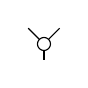
\begin{tikzpicture}[scale=0.2, black/.style={scale=0.5,draw,shape=circle,fill=white}]
	\node[black] (0) at (0, 0) {};
	\draw (1,1) to (0);
	\draw (-1,1) to (0);
	\draw (0) to (0,-1);
	\end{tikzpicture}
}

\newcommand{\counit}{
	\begin{tikzpicture}[scale=0.2, black/.style={scale=0.5,draw,shape=circle,fill=white}]
	\node[black] (0) at (0, 0) {};
	\draw (0) to (0,-1);
	\end{tikzpicture}
}

\newcommand{\antipode}{
	\begin{tikzpicture}[scale=0.2, black/.style={scale=0.5,draw,regular polygon,
		regular polygon sides=4,fill=white}]
	\node[scale=0.5, black] (0) at (0, 0) {$S$};
	\draw (0) to (0,-1);
	\draw (0) to (0,1);
	\end{tikzpicture}
}

\newcommand{\associativity}{
\begin{equation}
\begin{gathered}
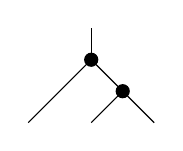
\begin{tikzpicture}[scale=0.8]
\node[scale=0.5,draw,circle,fill=black] (0) at (0,0.5) {};
\node[scale=0.5,draw,circle,fill=black] (1) at (0.5,0) {};
\draw (0) to (1);
\draw (-1,-0.5) to (0);
\draw (0,-0.5) to (1);
\draw (1,-0.5) to (1);
\draw (0) to (0,1);
\end{tikzpicture}
\end{gathered}
\, = \,
\begin{gathered}
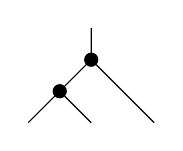
\begin{tikzpicture}[scale=0.8]
\node[scale=0.5,draw,circle,fill=black] (0) at (0.5,0.5) {};
\node[scale=0.5,draw,circle,fill=black] (1) at (0,0) {};
\draw (0) to (1);
\draw (-0.5,-0.5) to (1);
\draw (0.5,-0.5) to (1);
\draw (1.5,-0.5) to (0);
\draw (0) to (0.5,1);
\end{tikzpicture}
\end{gathered}
\end{equation}
}
\newcommand{\unitlaw}{
\begin{equation}
\begin{gathered}
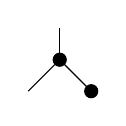
\begin{tikzpicture}[scale=0.8]
\node[scale=0.5,draw,circle,fill=black] (0) at (0,0.5) {};
\node[scale=0.5,draw,circle,fill=black] (1) at (0.5,0) {};
\draw (0) to (1);
\draw (-0.5,0) to (0);
\draw (0) to (0,1);
\end{tikzpicture}
\end{gathered}
\, = \,
\begin{gathered}
\begin{tikzpicture}[scale=0.8]
\draw (0,0) to (0,1);
\end{tikzpicture}
\end{gathered}
\, = \,
\begin{gathered}
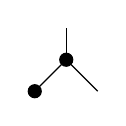
\begin{tikzpicture}[scale=0.8]
\node[scale=0.5,draw,circle,fill=black] (0) at (0,0.5) {};
\node[scale=0.5,draw,circle,fill=black] (1) at (-0.5,0) {};
\draw (0) to (1);
\draw (0.5,0) to (0);
\draw (0) to (0,1);
\end{tikzpicture}
\end{gathered}
\end{equation}
}
\newcommand{\coassociativity}{
\begin{equation}
\begin{gathered}
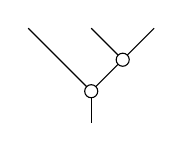
\begin{tikzpicture}[scale=0.8]
\node[scale=0.5,draw,circle,fill=white] (0) at (0,-0.5) {};
\node[scale=0.5,draw,circle,fill=white] (1) at (0.5,0) {};
\draw (0) to (1);
\draw (-1,0.5) to (0);
\draw (0,0.5) to (1);
\draw (1,0.5) to (1);
\draw (0) to (0,-1);
\end{tikzpicture}
\end{gathered}
\, = \,
\begin{gathered}
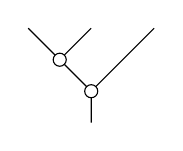
\begin{tikzpicture}[scale=0.8]
\node[scale=0.5,draw,circle,fill=white] (0) at (0.5,-0.5) {};
\node[scale=0.5,draw,circle,fill=white] (1) at (0,0) {};
\draw (0) to (1);
\draw (-0.5,0.5) to (1);
\draw (0.5,0.5) to (1);
\draw (1.5,0.5) to (0);
\draw (0) to (0.5,-1);
\end{tikzpicture}
\end{gathered}
\end{equation}
}
\newcommand{\counitlaw}{
\begin{equation}
\begin{gathered}
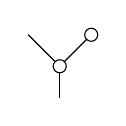
\begin{tikzpicture}[scale=0.8]
\node[scale=0.5,draw,circle,fill=white] (0) at (0,-0.5) {};
\node[scale=0.5,draw,circle,fill=white] (1) at (0.5,0) {};
\draw (0) to (1);
\draw (-0.5,0) to (0);
\draw (0) to (0,-1);
\end{tikzpicture}
\end{gathered}
\, = \,
\begin{gathered}
\begin{tikzpicture}[scale=0.8]
\draw (0,0) to (0,1);
\end{tikzpicture}
\end{gathered}
\, = \,
\begin{gathered}
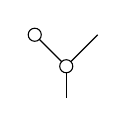
\begin{tikzpicture}[scale=0.8]
\node[scale=0.5,draw,circle,fill=white] (0) at (0,-0.5) {};
\node[scale=0.5,draw,circle,fill=white] (1) at (-0.5,0) {};
\draw (0) to (1);
\draw (0.5,0) to (0);
\draw (0) to (0,-1);
\end{tikzpicture}
\end{gathered}
\end{equation}
}

\newcommand{\bialgebralaw}{
\begin{equation}
\begin{gathered}
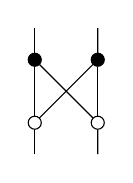
\begin{tikzpicture}[scale=0.8]
\node[scale=0.5,draw,circle,fill=white] (0) at (0,0) {};
\node[scale=0.5,draw,circle,fill=white] (1) at (1,0) {};
\node[scale=0.5,draw,circle,fill=black] (2) at (0,1) {};
\node[scale=0.5,draw,circle,fill=black] (3) at (1,1) {};
\draw (0) to (2);
\draw (0) to (3);
\draw (1) to (2);
\draw (1) to (3);
\draw (0,-0.5) to (0);
\draw (1,-0.5) to (1);
\draw (0,1.5) to (2);
\draw (1,1.5) to (3);
\end{tikzpicture}
\end{gathered}
\, = \,
\begin{gathered}
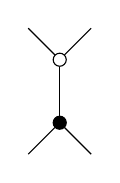
\begin{tikzpicture}[scale=0.8]
\node[scale=0.5,draw,circle,fill=black] (0) at (0.5,0) {};
\node[scale=0.5,draw,circle,fill=white] (1) at (0.5,1) {};
\draw (0) to (1);
\draw (0,-0.5) to (0);
\draw (1,-0.5) to (0);
\draw (0,1.5) to (1);
\draw (1,1.5) to (1);
\end{tikzpicture}
\end{gathered}
\end{equation}
}
\newcommand{\copylaw}{
\begin{equation}
\begin{gathered}
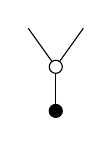
\begin{tikzpicture}[scale=0.7, squr/.style={scale=0.5,draw,regular polygon,
	regular polygon sides=4,fill=white}, black/.style={scale=0.5,draw,shape=circle,fill=black}, whit/.style={scale=0.5,draw,shape=circle,fill=white}]
\node[black] (0) at (0, 0) {};
\node[whit] (1) at  (0, 0.8) {};
\draw (0) to (1);
\draw (1) to (0.5,1.5);
\draw (1) to (-0.5,1.5);
\end{tikzpicture}
\end{gathered}
\, = \,
\begin{gathered}
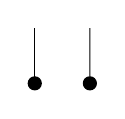
\begin{tikzpicture}[scale=0.7, black/.style={scale=0.5,draw,shape=circle,fill=black}]
\node[black] (0) at (0,0) {};
\node[black] (1) at (1,0) {};
\draw (0) to (0,1);
\draw (1) to (1,1);
\end{tikzpicture}
\end{gathered}
\end{equation}
}
\newcommand{\cocopylaw}{
	\begin{equation}
	\begin{gathered}
	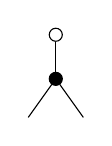
\begin{tikzpicture}[scale=0.7, squr/.style={scale=0.5,draw,regular polygon,
		regular polygon sides=4,fill=white}, black/.style={scale=0.5,draw,shape=circle,fill=black}, whit/.style={scale=0.5,draw,shape=circle,fill=white}]
	\node[whit] (0) at (0, 0) {};
	\node[black] (1) at  (0, -0.8) {};
	\draw (0) to (1);
	\draw (1) to (0.5,-1.5);
	\draw (1) to (-0.5,-1.5);
	\end{tikzpicture}
	\end{gathered}
	\, = \,
	\begin{gathered}
	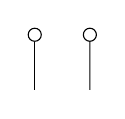
\begin{tikzpicture}[scale=0.7, black/.style={scale=0.5,draw,shape=circle,fill=white}]
	\node[black] (0) at (0,0) {};
	\node[black] (1) at (1,0) {};
	\draw (0) to (0,-1);
	\draw (1) to (1,-1);
	\end{tikzpicture}
	\end{gathered}
	\end{equation}
}
\newcommand{\hopflaw}{
	\begin{equation}
	\begin{gathered}
	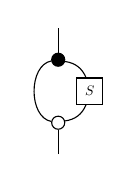
\begin{tikzpicture}[scale=0.8, squr/.style={scale=0.5,draw,regular polygon,
		regular polygon sides=4,fill=white}]
	\node[scale=0.5,draw,circle,fill=white] (0) at (0,0) {};
	\node[scale=0.5,draw,circle,fill=black] (1) at (0,1) {};
	\node[squr] (2) at (0.5,0.5) {$S$};
	\draw[bend left=80] (0) to (1);
	\draw[bend right] (0) to (2);
	\draw[bend right] (2) to (1);
	\draw (0,-0.5) to (0);
	\draw (0,1.5) to (1);
	\end{tikzpicture}
	\end{gathered}
	\, = \,
	\begin{gathered}
	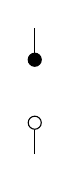
\begin{tikzpicture}[scale=0.8, squr/.style={draw,regular polygon,
		regular polygon sides=4,fill=white}]
	\node[scale=0.5,draw,circle,fill=white] (0) at (0,0) {};
	\node[scale=0.5,draw,circle,fill=black] (1) at (0,1) {};
	\draw (0,-0.5) to (0);
	\draw (0,1.5) to (1);
	\end{tikzpicture}
	\end{gathered}
	\, = \,
	\begin{gathered}
	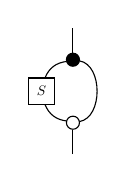
\begin{tikzpicture}[scale=0.8, squr/.style={scale=0.5,draw,regular polygon,
		regular polygon sides=4,fill=white}]
	\node[scale=0.5,draw,circle,fill=white] (0) at (0,0) {};
	\node[scale=0.5,draw,circle,fill=black] (1) at (0,1) {};
	\node[squr] (2) at (-0.5,0.5) {$S$};
	\draw[bend right=80] (0) to (1);
	\draw[bend left] (0) to (2);
	\draw[bend left] (2) to (1);
	\draw (0,-0.5) to (0);
	\draw (0,1.5) to (1);
	\end{tikzpicture}
	\end{gathered}
	\end{equation}
}
\newcommand{\modulelaw}{
	\begin{equation}
	\begin{gathered}
	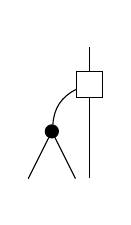
\begin{tikzpicture}[scale=0.6, squr/.style={draw,regular polygon,
		regular polygon sides=4,fill=white}, black/.style={scale=0.5,draw,shape=circle,fill=black}]
	\node (0) at (0, -2.2) {};
	\node[squr] (1) at (0, 0) {};
	\node (2) at (0, 1) {};
	\node[black] (3) at (-0.8, -1) {};
	\draw (0) to (1);
	\draw (1) to (2);
	\draw[bend left] (3) to (1);
	\draw (-1.3, -2) to (3);
	\draw (-0.3, -2) to (3);
	\end{tikzpicture}
	\end{gathered}
	\, = \,
	\begin{gathered}
	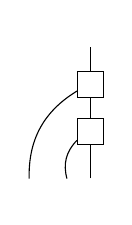
\begin{tikzpicture}[scale=0.6, squr/.style={draw,regular polygon,
		regular polygon sides=4,fill=white}, black/.style={draw,shape=circle,fill=black}]
	\node (0) at (0, -2.2) {};
	\node[squr] (1) at (0, 0) {};
	\node (2) at (0, 1) {};
	\node[squr] (3) at (0, -1) {};
	\draw (0) to (3);
	\draw (3) to (1);
	\draw (1) to (2);
	\draw (3) to (1);
	\draw[bend left] (-1.3, -2) to (1);
	\draw[bend left] (-0.5, -2) to (3);
	\end{tikzpicture}
	\end{gathered}
	\end{equation}
}
\newcommand{\intertwinerlaw}{
\begin{equation}
\begin{gathered}
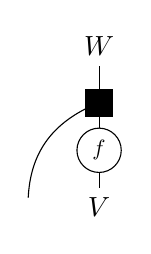
\begin{tikzpicture}[scale=0.6, squr/.style={draw,regular polygon,
	regular polygon sides=4,fill=black}]
\node (0) at (0, -2.2) {$V$};
\node[squr] (1) at (0, 0) {};
\node (2) at (0, 1.2) {$W$};
\node[scale=0.8,draw,circle] (3) at (0, -1) {$f$};
\draw (0) to (3);
\draw (3) to (1);
\draw (1) to (2);
\draw (3) to (1);
\draw[bend left] (-1.5, -2) to (1);
\end{tikzpicture}	
\end{gathered}
\, = \,
\begin{gathered}
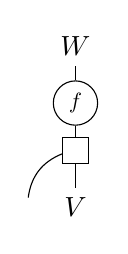
\begin{tikzpicture}[scale=0.6, squr/.style={draw,regular polygon,
	regular polygon sides=4,fill=white}]
\node (0) at (0, -2.2) {$V$};
\node[scale=0.8,draw,circle] (1) at (0, 0) {$f$};
\node (2) at (0, 1.2) {$W$};
\node[squr] (3) at (0, -1) {};
\draw (0) to (3);
\draw (3) to (1);
\draw (1) to (2);
\draw (3) to (1);
\draw[bend left] (-1, -2) to (3);
\end{tikzpicture}	
\end{gathered}
\end{equation}
}
\newcommand{\symAB}{
	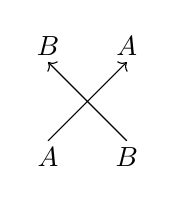
\begin{tikzpicture}[decoration={markings,mark=at position 0.5 with {\arrow{>}}}]
	\node (0) at (-0.5, -0.7) {$A$};
	\node (0) at (-0.5, 0.7) {$B$};
	\node (1) at (0.5, -0.7) {$B$};
	\node (1) at (0.5, 0.7) {$A$};
	\draw [->] (-0.5, -0.5) to (0.5, 0.5);
	\draw [->] (0.5, -0.5) to (-0.5, 0.5);
	\end{tikzpicture}
}

\newcommand{\symequation}{
	\begin{equation*}
	\begin{gathered}
	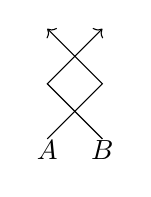
\begin{tikzpicture}[scale=0.7]
	\node (0) at (-1, -1.2) {$A$};
	\node (0) at (0, -1.2) {$B$};
	\draw [->] (-1, -1)--(0,0)--(-1,1);
	\draw [->] (0, -1)--(-1,0)--(0,1);
	\end{tikzpicture}
	\end{gathered}
	\, = \,
	\begin{gathered}
	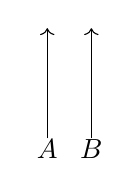
\begin{tikzpicture}[scale=0.7]
	\node (0) at (-0.8, -1.2) {$A$};
	\node (0) at (0, -1.2) {$B$};
	\draw [->] (-0.8, -1)--(-0.8,1);
	\draw [->] (0, -1)--(0,1);
	\end{tikzpicture}
	\end{gathered}
	\end{equation*}
}

\newcommand{\cupA}{	
	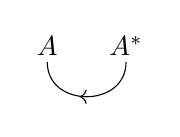
\begin{tikzpicture}[decoration={markings,mark=at position 0.5 with {\arrow{<}}}]
	\node (0) at (0, 0.2) {$A$};
	\node (1) at (1, 0.2) {$A^*$};
	\draw [bend right=90, looseness=1.5, postaction=decorate] (0,0) to (1,0);
	\end{tikzpicture}}

\newcommand{\capA}{	
	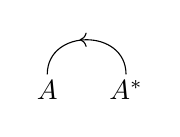
\begin{tikzpicture}[decoration={markings,mark=at position 0.5 with {\arrow{<}}}]
	\node (0) at (0, -0.2) {$A$};
	\node (1) at (1, -0.2) {$A^*$};
	\draw [bend left=90, looseness=1.5, postaction=decorate] (0,0) to (1,0);
	\end{tikzpicture}}

\newcommand{\snake}{
	\begin{equation*}
	\begin{gathered}
	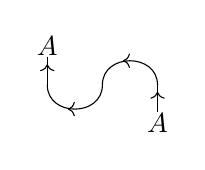
\begin{tikzpicture}[scale=0.7,decoration={markings,mark=at position 0.5 with {\arrow{<}}}]
	\node (0) at (0, 0.7) {$A$};
	\node (4) at (2, -0.7){$A$};
	\draw [bend right=90, looseness=1.5, postaction=decorate] (0, 0) to (1, 0);
	\draw [bend left=90, looseness=1.5, postaction=decorate] (1, 0) to (2, 0);
	\draw [postaction=decorate] (2, 0) to (2, -0.5);
	\draw [postaction=decorate] (0, 0.5) to (0, 0);
	\end{tikzpicture}
	\end{gathered}
	\, = \,
	\begin{gathered}
	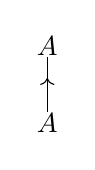
\begin{tikzpicture}[scale=0.7,decoration={markings,mark=at position 0.5 with {\arrow{<}}}]
	\node (0) at (0, 0.7) {$A$};
	\node (4) at (0, -0.7){$A$};
	\draw [postaction=decorate] (0, 0.5) to (0, -0.5);
	\end{tikzpicture}
	\end{gathered}
	\end{equation*}}

\newcommand{\snakestar}{
	\begin{equation*}
	\begin{gathered}
	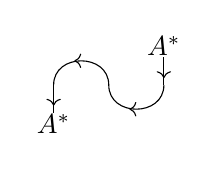
\begin{tikzpicture}[scale=0.7,decoration={markings,mark=at position 0.5 with {\arrow{<}}}]
	\node (0) at (0, -0.7) {$A^*$};
	\node (4) at (2, 0.7){$A^*$};
	\draw [bend left=90, looseness=1.5, postaction=decorate] (0, 0) to (1, 0);
	\draw [bend right=90, looseness=1.5, postaction=decorate] (1, 0) to (2, 0);
	\draw [postaction=decorate] (2, 0) to (2, 0.5);
	\draw [postaction=decorate] (0, -0.5) to (0, 0);
	\end{tikzpicture}
	\end{gathered}
	\, = \,
	\begin{gathered}
	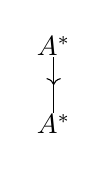
\begin{tikzpicture}[scale=0.7,decoration={markings,mark=at position 0.5 with {\arrow{>}}}]
	\node (0) at (0, 0.7) {$A^*$};
	\node (4) at (0, -0.7){$A^*$};
	\draw [postaction=decorate] (0, 0.5) to (0, -0.5);
	\end{tikzpicture}
	\end{gathered}
	\end{equation*}
}

\newcommand{\fusionijk}{
	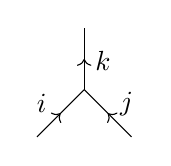
\begin{tikzpicture}[scale=0.6,decoration={markings,mark=at position 0.5 with {\arrow{>}}}]
	\node (0) at (-0.9, -0.3) {$i$};
	\node (1) at (0.9, -0.3) {$j$};
	\node (2) at (0.4, 0.6) {$k$};
	\draw [postaction=decorate] (-1, -1) to(0,0);
	\draw [postaction=decorate] (1,-1) to (0,0);
	\draw [postaction=decorate] (0,0) to (0,1.3);
	\end{tikzpicture}}
%%%%%%%%%%%%%%%%%%%%%%%%%%%%%%%%%%%%%%%%%%%%%%%%%%%%%%%%%%%%%%%%%%%%%%%%%%%%%%%%%%%%%%%%%%%%%%%%%%%%%%%%%%%%%%%%%%%%%%%%%%%%%%%%%%%%%%%%%%%%%%%%%%%%%%%%%%%%%%%%%%%%%%%%%%%%%%%%%%%%


\begin{document}

%%%%%%%%%%%%%%%%%%%%%%%%%%%%%%%%%%%%%%%%%%%%%%%%%%%%%%%%%%%%%%%%%%%%%%%%%%%%%%%%%%%%%%%%%%%%%%%%%%%%%%%%%%%%%%%%%%%%%%%%%%%%%%%%%%%%%%%%%%%%%%%%
%%%%%%%%%%%%%%%%%%%%%%%%%%%%%%%%%%%%%%%%%%%%%%%%%%%%%%%%%%%%%%%%%%%%%%%%%%%%%%%%%%%%%%%%%%%%%%%%%%%%%%%%%%%%%%%%%%%%%%%%%%%%%%%%%%%%%%%%%%%%%%%%
%%%%%%%%%%%%%%%%%%%%%%%%%%%%%%%%%%%%%%%%%%%%%%%%%%%%%%%%%%%%%%%%%%%%%%%%%%%%%%%%%%%%%%%%%%%%%%%%%%%%%%%%%%%%%%%%%%%%%%%%%%%%%%%%%%%%%%%%%%%%%%%%
%%%%%%%%%%%%%%%%%%%%%%%%%%%%%%%%%%%%%%%%%%%%%%%%%%%%%%%%%%%%%%%%%%%%%%%%%%%%%%%%%%%%%%%%%%%%%%%%%%%%%%%%%%%%%%%%%%%%%%%%%%%%%%%%%%%%%%%%%%%%%%%%

\section{Diagrams and Hopf Algebras}



\subsection{Monoidal categories}
In this section, we set in place the basic definitions and diagrammatic  intuitions which we will use throughout the thesis. The standard reference about basic category theory results is \cite{MacLane71}. Many of the definitions are taken from \cite{Abramsky11}. A more detailed and up to date survey on monoidal categories can be found in \cite{Etingof15}. For an introduction to diagrammatic reasoning in monoidal categories consider the first two chapters of \cite{Coecke17}. Many of the results in this section and their relationship to quantum mechanics can be found in \cite{Vicary12}. \\
%%CATEGORIES:
Recall the definition of a category.
\begin{definition}
	A category $\cat$ consists of the data:
	\begin{itemize}
		\item a collection of objects $obj(\cat)$ 
		\item a collection of morphisms (or arrows) $arr(\cat)$
		\item domain and codomain assignments $dom, cod: arr(\cat) \rightarrow obj(\cat)$. For any two objects $a,b \in obj(\cat)$ we define the hom-set 
		$$ \cat (a,b) := \{ f \in arr(\cat) : a= dom(f), b=cod(f) \}$$
		\item for any triple of objects $a,b,c$ a composition map 
		$$c_{a,b,c}: \cat (a,b) \times \cat (b,c) \rightarrow \cat (a,c)$$
		We denote the composition by $g \circ f$, diagrammatically:
		\begin{center}
			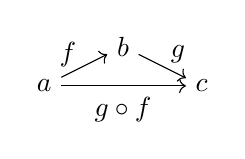
\begin{tikzpicture}
			\node (0) at (-1, 0) {$a$};
			\node (1) at (0, 0.5) {$b$};
			\node (2) at (1, 0) {$c$};
			\node (3) at (-0.7, 0.4) {$f$};
			\node (3) at (0.7, 0.4) {$g$};
			\node (3) at (0, -0.3) {$g\circ f$};
			\draw [->] (0) to (1);
			\draw [->] (1) to (2);
			\draw [->] (0) to (2);
			\end{tikzpicture}
		\end{center}
		\item For any object $a$ an identity morphism $id_a: a \rightarrow a$ 
	\end{itemize}
	Satisfying the following axioms:
	\begin{equation*}
	h \circ (g \circ f) = (h \circ g) \circ f \quad f \circ id_a = f = id_b \circ f
	\end{equation*}
	
\end{definition}
\begin{center}
	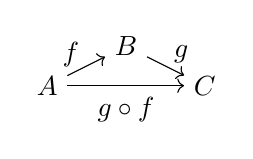
\begin{tikzpicture}
	\node (0) at (-1, 0) {$A$};
	\node (1) at (0, 0.5) {$B$};
	\node (2) at (1, 0) {$C$};
	\node (3) at (-0.7, 0.4) {$f$};
	\node (3) at (0.7, 0.4) {$g$};
	\node (3) at (0, -0.3) {$g\circ f$};
	\draw [->] (0) to (1);
	\draw [->] (1) to (2);
	\draw [->] (0) to (2);
	\end{tikzpicture}
\end{center}
The commutativity of the above diagram is a statement about $\cat$, and it has exactly the same information to its dual diagram. Where objects are one-dimensional wires and morphisms are (zero dimensional) boxes:
\begin{center}
	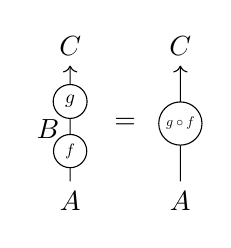
\begin{tikzpicture}[scale=0.7]
	\node (0) at (-1, -1.4) {$A$};
	\node (1) at (-1.4, -0.1) {$B$};
	\node (2) at (-1, 1.4) {$C$};
	\node (3) at (1, -1.4) {$A$};
	\node (4) at (1, 1.4) {$C$};
	\node[scale=0.6,draw,circle] (5) at (-1, -0.5) {$f$};
	\node[scale=0.7,draw,circle] (6) at (-1, 0.4) {$g$};
	\node[scale=0.5,draw,circle] (7) at (1, 0) {$g\circ f$};
	\node (8) at (0, 0) {$=$};
	\draw (0) to (5);
	\draw (5) to (6);
	\draw [->] (6) to (2);
	\draw (3) to (7);
	\draw [->] (7) to (4);
	\end{tikzpicture}
\end{center}
We will mainly use this second diagrammatic language in this work. When $\cat$ is just a category we only have one way of composing morphisms and the language is one dimensional.
\begin{example}
	Examples of categories are: $Sets$ of sets and functions, $FSets$ of finite sets and functions, $Rel$ of sets and relations, $Vect_k$ of vector spaces over $k$ and linear maps and $FVect_k$ of finite dimensional vector spaces and linear maps.
\end{example}
Category theory is a really good language for talking about equivalences and relationships between structures. This is achieved with the following tools.
\begin{definition}[Functor]
	A functor $F:\mathcal{C} \rightarrow \mathcal{D}$ is a mapping that
	\begin{itemize}
		\item associates an object $F(X)$ of $\mathcal{D}$ to each object $X$ of $\mathcal{C}$.
		\item associates to each morphism $f:X \rightarrow Y$ a morphism $F(f): F(X) \rightarrow F(Y)$ such that $F(id_X)=id_Y$ and $F(g\circ f)= F(g)\circ F(f)$ for all morphisms $f:X \rightarrow Y$ and $g:Y \rightarrow Z$.
	\end{itemize}
\end{definition}
For instance there is a functor $Q: Sets \rightarrow Vect_k$ called `1st quantization' and taking a set to the free vector space generated by that set.
Given two functors with matching source and target we can have natural transformations between them
\begin{definition}[Natural Transformation]
	Given categories $\cat$ and $\mathcal{D}$ and functors $F,G:\cat \rightarrow \mathcal{D}$ a natural transformation $\alpha: F \Rightarrow G$ is an assignment to every object $a$ in $\cat$ of a morphism $\alpha_a:F(a) \rightarrow G(a)$ in $\mathcal{D}$ such that for each morphism $f:a \rightarrow b$, the following commutes:
	\begin{center}
		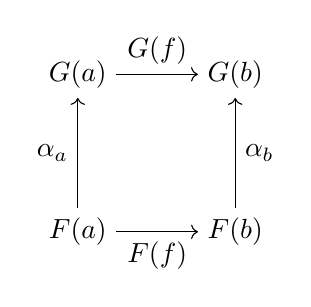
\begin{tikzpicture}[scale=2]
		\node (0) at (0,0) {$F(a)$};
		\node (1) at (0,1) {$G(a)$};
		\node (3) at (1,0) {$F(b)$};
		\node (4) at (1,1) {$G(b)$};
		\draw [->] (0)--(1) node[midway,left] {$\alpha_a$};
		\draw [->] (3)--(4) node[midway,right] {$\alpha_b$};
		\draw [->] (0)--(3) node[midway,below] {$F(f)$};
		\draw [->] (1)--(4) node[midway,above] {$G(f)$};
		\end{tikzpicture}
	\end{center}
	A natural isomorphism is a natural transformation such that all components are isomorphisms.
\end{definition}
%%%MONOIDAL CATEGORIES:
Recall that a monoid is a triple $(X, \times, 1)$ where $X$ is a set, $1 \in X$ and $\times$ is an associative and unital multiplication on $X$. The notion of a monoidal category is the categorification of a monoid. Elements of the set are replaced by objects in a category $\mathcal{C}$, multiplication by a bifunctor $\otimes: \mathcal{C} \times \mathcal{C} \rightarrow \mathcal{C}$ and the equalities in the unit and association axioms are replaced by natural isomorphisms. In order for this new structure to be well-behaved we will also need to impose compatibility conditions. We obtain the following definition:
\begin{definition}[Monoidal category]
	A monoidal category is a category $\mathcal{C}$ equipped with a bifunctor $\otimes: \mathcal{C} \times \mathcal{C} \rightarrow \mathcal{C}$ called tensor product, an object $1$ called unit object, a natural isomorphism
	$$ a : -\otimes(- \otimes -) \xRightarrow{\sim} (-\otimes -) \otimes -$$ called associator, a natural isomorphism 
	$$\lambda: 1 \otimes (-) \Rightarrow (-)$$ called left unitor and a natural isomorphism
	$$ \rho: (-) \otimes 1 \Rightarrow (-)$$
	called right unitor. Subject to the following coherence conditions holding for all objects $a,b,c,d$ in $\mathcal{C}$:
	\begin{enumerate}
		\item Pentagon axiom: the following diagram commutes
		\begin{center}
			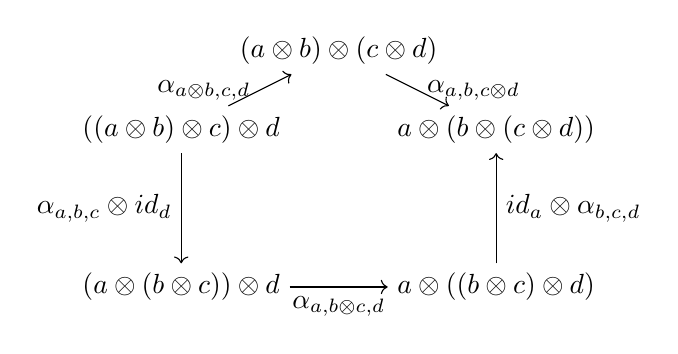
\begin{tikzpicture}[scale=2]
			\node (0) at (0,0) {$(a\otimes (b \otimes c)) \otimes d$};
			\node (1) at (0,1) {$((a\otimes b) \otimes c) \otimes d$};
			\node (2) at (1,1.5) {$(a\otimes b) \otimes (c \otimes d)$};
			\node (3) at (2,1) {$a\otimes (b \otimes (c \otimes d))$};
			\node (4) at (2,0) {$a\otimes ((b \otimes c) \otimes d)$};
			\draw [->] (1)--(2) node[midway,left] {$\alpha_{a \otimes b,c,d}$};
			\draw [->] (2)--(3) node[midway,right] {$\alpha_{a, b,c \otimes d}$};
			\draw [->] (1)--(0) node[midway,left] {$\alpha_{a, b,c} \otimes id_d$};
			\draw [->] (0)--(4) node[midway,below] {$\alpha_{a,b \otimes c,d}$};
			\draw [->] (4)--(3) node[midway,right] {$id_a \otimes \alpha_{b,c,d}$};
			\end{tikzpicture}
		\end{center}
		\item Triangle identity: the following diagram commutes
		\begin{center}
			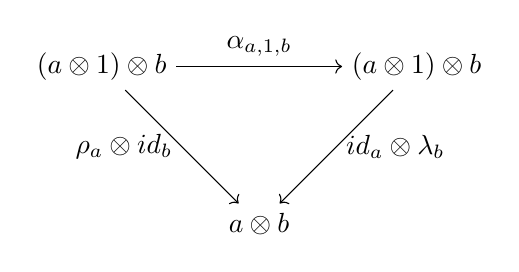
\begin{tikzpicture}[scale=2]
			\node (0) at (0,0) {$(a\otimes 1) \otimes b$};
			\node (1) at (2,0) {$(a\otimes 1) \otimes b$};
			\node (2) at (1,-1) {$a\otimes b$};
			\draw [->] (0)--(1) node[midway,above] {$\alpha_{a ,1,b}$};
			\draw [->] (1)--(2) node[midway,right] {$id_a \otimes \lambda_b$};
			\draw [->] (0)--(2) node[midway,left] {$\rho_a \otimes id_b$};
			\end{tikzpicture}
		\end{center}
	\end{enumerate}
\end{definition}
Let us give three important examples of monoidal categories.
\begin{example}
	The category $Sets$ of sets and functions is monoidal with the cartesian product $\times$ as bifunctor and the singleton set as unit object.\\
	The category $Vect_k$ of finite dimensional vector spaces over a field $k$ is monoidal with the usual tensor product $\otimes$ and the one dimensional vector space $k$ as unit object.\\
	The category $Rel$ of sets and relations is monoidal with the cartesian product $\times$ and the singleton as unit object.
\end{example}
The more structure comes with a category the more complicated diagrams we can draw. Monoidal categories have a two-dimensional diagrammatic language. The presence of unitors and associators and the conditions they satisfy make sure that this graphical language is well behaved. This is known as the coherence theorem for monoidal categories and can be found in \cite{MacLane71}. It says that any well formed diagram in a monoidal category, made up of associators and unitors commutes. When the associators are trivial morphisms (i.e identity morphisms) we say the category is strict monoidal. It is known that every monoidal category is equivalent to a strict one \cite{MacLane71}, but it is sometimes useful to take associators into account as we will see in our discussion on permutational quantum computation.\\
We write the tensor of two morphisms $f \otimes g : A \otimes B \rightarrow C \otimes D$ simply putting them side by side:
\begin{center}
	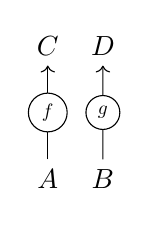
\begin{tikzpicture}[scale=0.7]
	\node (0) at (0, -1.2) {$A$};
	\node (1) at (1, -1.2) {$B$};
	\node (2) at (0, 1.2) {$C$};
	\node (3) at (1, 1.2) {$D$};
	\node[scale=0.7,draw,circle] (5) at (0, 0) {$f$};
	\node[scale=0.7,draw,circle] (6) at (1, 0) {$g$};
	\draw (0) to (5);
	\draw [->] (5) to (2);
	\draw (1) to (6);
	\draw [->] (6) to (3);
	\end{tikzpicture}
\end{center}
In our diagrams we can picture the unit $I$ of the tensor as the plane on which we are drawing. Indeed we could imagine drawing as many copies as we wanted of $id_I$ on the previous diagram to obtain obtain an equivalent diagram as $id_I \otimes f = f$ for any morphism $f$. So really the identity on $I$ is just the empty diagram which we can stick next to any diagram we like.
\begin{definition}[States and costates]
	Given a system $A$, a state of is a morphism $1 \rightarrow A$. A costate (or effect) of $A$ is a morphism $A \rightarrow 1$. In the diagrammatic language we draw states and costates respectively:
	\begin{center}
		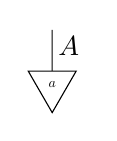
\begin{tikzpicture}[scale=0.7]
		\node[scale=0.5,buffer] (1) {$a$}; 
		\node (2) at (0.3,0.7) {$A$};
		\draw (1)--(0,1);
		\end{tikzpicture}
		\quad \quad
		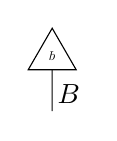
\begin{tikzpicture}[scale=0.7]
		\node[scale=0.5,buffer,rotate=180] (1) at (0,0) {$q$}; 
		\node (2) at (0.3,-0.7) {$B$};
		\draw (1)--(0,-1);
		\end{tikzpicture}
	\end{center}
	
	
\end{definition}


%%%DIAGRAMS:
\begin{remark}
	It is perhaps useful to understand monoidal categories as degenerate 2-categories. Although this viewpoint requires one additional initial step of abstraction (the definition of a 2-category), it gives us the diagrammatic language for monoidal categories for free. For the rigorous definition of a 2-category we refer to [BAEZ], for our purposes we will only need the intuition. A 2-category is a collection of objects with 1-arrows between them and 2-arrows between the 1-arrows. Note that there are two ways of composing the 2-arrows:
	\begin{itemize}
		\item vertical composition:
		\begin{center}
			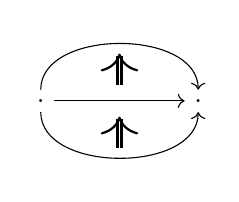
\begin{tikzpicture}
			\node (0) at (0,0) {.};
			\node (1) at (2,0) {.};
			\draw[->] (0) to (1);
			\draw[->, bend right=90] (0) to (1);
			\draw[->, bend left=90] (0) to (1);
			\draw[double, thick, ->] (1,-0.6) to (1,-0.2);
			\draw[double, thick, ->] (1,0.2) to (1,0.6);
			\end{tikzpicture}
		\end{center}
		\item parallel composition:
		\begin{center}
			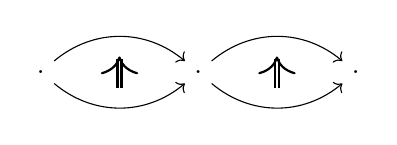
\begin{tikzpicture}
			\node (0) at (0,0) {.};
			\node (1) at (2,0) {.};
			\node (2) at (4,0) {.};
			\draw[->, bend right=40] (0) to (1);
			\draw[->, bend left=40] (0) to (1);
			\draw[->, bend right=40] (1) to (2);
			\draw[->, bend left=40] (1) to (2);
			\draw[double, thick, ->] (1,-0.2) to (1,0.2);
			\draw[double, thick, ->] (3,-0.2) to (3,0.2);
			\end{tikzpicture}
		\end{center}
	\end{itemize}
	Taking the dual of the above diagrams we obtain the diagrammatic language. Monoidal categories are 2-categories with only one 0-object called $1$. We can think of the 0-object as the underlying plane, wires carry systems (1-arrows), boxes are morphisms (2-arrows). We recover the given definition of monoidal category by calling 1-arrow objects, and 2-arrows morphisms. The unit object $1$ is then the identity 1-arrow $1 \rightarrow 1$ which is simply denoted $1$.
\end{remark}

\begin{example}
	The cartesian product in $Sets$ $A \times B$ of sets $A$ and $B$, satisfies the universal properties of a categorical product, in the sense that we have projections $p_1$ and $p_2$ such that if $f$ and $g$ are maps from some set $C$ there is a unique function $h$ making the following diagram commute:
	\begin{center}
		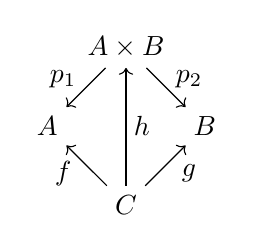
\begin{tikzpicture}
		\node (0) at (-1, 0) {$A$};
		\node (1) at (1, 0) {$B$};
		\node (2) at (0, 1) {$A \times B$};
		\node (3) at (0, -1) {$C$};
		\node (4) at (0.2, 0) {$h$};
		\node (5) at (-0.8, 0.6) {$p_1$};
		\node (6) at (0.8, 0.6) {$p_2$};
		\node (7) at (-0.8, -0.6) {$f$};
		\node (8) at (0.8, -0.6) {$g$};
		\draw [->] (2) to (0);
		\draw [->] (2) to (1);
		\draw [->] (3) to (1);
		\draw [->] (3) to (0);
		\draw [->] (3) to (2);
		\end{tikzpicture}
	\end{center}
	Because of this property all states of $(Sets,\times)$ are separable. This category is the ambient Cartesian world of classical physics.
\end{example}
\begin{example}
	In $Vect_k$ states are vectors and costates are functionals. Note that the diagrammatic notation provides a two-dimensional generalisation of Dirac's notation. The category $Hilb$ of Hilbert spaces and linear maps is monoidal when equipped with the usual tensor product $\otimes$. Note that $\otimes$ is not a categorical product, and in fact we can have entangled states. Quantum mechanics is based on $(Hilb, \otimes)$ \cite{Vicary12}.
\end{example}
\begin{definition}[Scalars]
	Scalars in a monoidal category are morphisms $1 \rightarrow 1$.
\end{definition}
The category $Sets$ has only one scalar. $Rel$ has two scalars forming the cyclic group $\mathbb{Z}_2$ under composition. $Vect_k$ has scalars from $k$. Given a vector and a functional we obtain a scalar by composing them analogously to Dirac's formalism.
\begin{definition}[BMC]
	A braided monoidal category is a monoidal category $\mathcal{C}$ equipped with a natural isomorphism $B_{a,b} : a \otimes b \rightarrow b \otimes a$ called braiding, subject to the following compatibility conditions (called hexagon equations):
	\begin{center}
		\begin{tikzpicture}[scale=2]
		\node (0) at (-1,0) {$(a\otimes b) \otimes c$};
		\node (1) at (-0.5,1) {$a\otimes (b \otimes c)$};
		\node (2) at (1.5,1) {$(b\otimes c)\otimes a$};
		\node (3) at (2,0) {$b\otimes (c\otimes a)$};
		\node (4) at (-0.5,-1) {$(b\otimes a)\otimes c$};
		\node (5) at (1.5,-1) {$b\otimes (a\otimes c)$};
		\draw [->] (0)--(1) node[midway,left] {$\alpha_{a,b,c}$};
		\draw [->] (1)--(2) node[midway,above] {$B_{a,b \otimes c}$};
		\draw [->] (2)--(3) node[midway,right] {$\alpha_{b,c,a}$};
		\draw [->] (0)--(4) node[midway,left] {$B_{a,b} \otimes id_c$};
		\draw [->] (4)--(5) node[midway,below] {$\alpha_{b,a,c}$};
		\draw [->] (5)--(3) node[midway,right] {$id_b \otimes B_{a,c}$};
		\end{tikzpicture}
	\end{center}
	\begin{center}
		\begin{tikzpicture}[scale=2]
		\node (0) at (-1,0) {$a\otimes (b \otimes c)$};
		\node (1) at (-0.5,1) {$(a\otimes b) \otimes c$};
		\node (2) at (1.5,1) {$c\otimes (a\otimes b)$};
		\node (3) at (2,0) {$(c\otimes a)\otimes b$};
		\node (4) at (-0.5,-1) {$a\otimes (c\otimes b)$};
		\node (5) at (1.5,-1) {$(a\otimes c)\otimes b$};
		\draw [->] (0)--(1) node[midway,left] {$\alpha_{a,b,c}$};
		\draw [->] (1)--(2) node[midway,above] {$B_{a\otimes b,c}$};
		\draw [->] (2)--(3) node[midway,right] {$\alpha_{c,a,b}$};
		\draw [->] (0)--(4) node[midway,left] {$id_a \otimes B_{b,c}$};
		\draw [->] (4)--(5) node[midway,below] {$\alpha_{a,c,b}$};
		\draw [->] (5)--(3) node[midway,right] {$B_{a,c} \otimes id_b$};
		\end{tikzpicture}
	\end{center}
	
\end{definition}
In the diagrammatic language this means we have braidings:
\begin{center}
	\begin{tikzpicture}[scale=0.9, whit/.style={draw,regular polygon,
		regular polygon sides=4,fill=white}, black/.style={draw,regular polygon, regular polygon sides=4,fill=black}]
	\node (0) at (0.5,0.5) {};
	\node (1) at (-0.1,-0.4) {$A$};
	\node (2) at (1.1,-0.4) {$B$};
	\draw (0,1) to (1,0);
	\draw (0,0) to (0);
	\draw (0) to (1,1);
	\end{tikzpicture}
	\begin{tikzpicture}[scale=0.9, whit/.style={draw,regular polygon,
		regular polygon sides=4,fill=white}, black/.style={draw,regular polygon, regular polygon sides=4,fill=black}]
	\node (0) at (0.5,0.5) {};
	\node (1) at (-0.1,-0.4) {$B$};
	\node (2) at (1.1,-0.4) {$A$};
	\draw (0,0) to (1,1);
	\draw (0,1) to (0);
	\draw (0) to (1,0);
	\end{tikzpicture}
\end{center}
for any $A$ and $B$, satifying:
\begin{equation}
\begin{gathered}
\begin{tikzpicture}[scale=0.6, whit/.style={draw,regular polygon,
	regular polygon sides=4,fill=white}, black/.style={draw,regular polygon, regular polygon sides=4,fill=black}]
\node (0) at (0.5,0.5) {};
\node (1) at (-0.1,-0.4) {$A$};
\node (2) at (1.1,-0.4) {$B$};
\node (3) at (0.5,1.5) {};
\draw (1,0)--(0,1)--(1,2);
\draw (0,0)--(0)--(1,1)--(3)--(0,2);
\end{tikzpicture}
\end{gathered}
\, = \,
\begin{gathered}
\begin{tikzpicture}[scale=0.6, whit/.style={draw,regular polygon,
	regular polygon sides=4,fill=white}, black/.style={draw,regular polygon, regular polygon sides=4,fill=black}]
\node (1) at (0,-0.4) {$A$};
\node (2) at (0.9,-0.4) {$B$};
\draw (0.8,0)--(0.8,2);
\draw (0.1,0)--(0.1,2);
\end{tikzpicture}
\end{gathered}
\quad;\quad
\begin{gathered}
\begin{tikzpicture}[scale=0.6, whit/.style={draw,regular polygon,
	regular polygon sides=4,fill=white}, black/.style={draw,regular polygon, regular polygon sides=4,fill=black}]
\node (0) at (0.5,0.5) {};
\node (1) at (-0.1,-0.4) {$B$};
\node (2) at (1.1,-0.4) {$A$};
\node (3) at (0.5,1.5) {};
\draw (1,0)--(0)--(0,1)-- (3)--(1,2);
\draw (0,0)--(1,1)--(0,2);
\end{tikzpicture}
\end{gathered}
\, = \,
\begin{gathered}
\begin{tikzpicture}[scale=0.6, whit/.style={draw,regular polygon,
	regular polygon sides=4,fill=white}, black/.style={draw,regular polygon, regular polygon sides=4,fill=black}]
\node (1) at (0,-0.4) {$B$};
\node (2) at (0.9,-0.4) {$A$};
\draw (0.8,0)--(0.8,2);
\draw (0.1,0)--(0.1,2);
\end{tikzpicture}
\end{gathered}
\end{equation}
The compatibility conditions are obvious statements in the diagrammatic calculus, for instance the first hexagon equation just says:
\begin{equation}
\begin{gathered}
\begin{tikzpicture}[scale=0.6]
\node (0) at (0.5,0.5) {};
\node (1) at (-0.1,-0.4) {$A$};
\node (2) at (1.1,-0.4) {$B$};
\node (3) at (2.1,-0.4) {$C$};
\node (4) at (1.5,2.5) {};
\draw (0,0)--(1,1)--(1,2)--(2,3);
\draw (1,0)--(0)--(0,1)--(0,3);
\draw (2,0)--(2,2)--(4)--(1,3);
\end{tikzpicture}
\end{gathered}
\, = \,
\begin{gathered}
\begin{tikzpicture}[scale=0.6]
\node (0) at (1.3,2.2) {};
\node (1) at (0.4,-0.4) {$A$};
\node (2) at (1.5,-0.4) {$B$};
\node (3) at (2.2,-0.4) {$C$};
\node (4) at (1.5,2.5) {};
\draw (0.5,0)--(0.5,1.5)--(1,2)--(2,3);
\draw (1.7,0)--(1.7,1.7)--(0)--(0.5,3);
\draw (2,0)--(2,2)--(4)--(1,3);
\end{tikzpicture}
\end{gathered}
\end{equation}
Both $Sets$ and $Hilb$ are examples of symmetric monoidal categories in the following sense.
\begin{definition}[SMC]
	A braided monoidal category is symmetric if the braiding $B_{a,b}$ satisfies $$B_{a,b} \circ B_{b,a} = id_{a\otimes b}$$
	For all objects $a,b$
\end{definition}
In a SMC the braiding is called symmetry morphism and is denoted
\begin{center}
	\symAB	
\end{center}
It satisfies:
\symequation
We will now describe some new classes of examples of monoidal categories. These are of a different nature to the categories we have seen so far.
\begin{definition}[PROPs]
	A $PROP$ (products and permutations category) is a strict symmetric monoidal category where every object is of the form $x^{\otimes n}$ for a single object $x$ and $n \geq 0$.
\end{definition}
This means that we are only allowed one type of wire when drawing diagrams about $PROPs$ but we can use as many copies as we like and we can make swaps with them. Categories satisfying these properties are useful syntactic tools as we will see.
One way to think of a $PROP$ $A$ is as an abstract algebraic structure carrying some axioms, we can then instantiate those axioms in some other symmetric monoidal category $\mathcal{C}$ by considering symmetric monoidal functors $F: A \rightarrow \mathcal{C}$. We call such functors algebras or models of $A$ in $\mathcal{C}$. If $A$ is defined in terms of generators and relations (as is most often done), the choice of such functor corresponds to the choice of one object from $\mathcal{C}$ and morphisms on that object respecting the defining relations of $A$. On its own $A$ has no clear interpretation, it just defines a syntax, but if $\mathcal{C}$ is a semantic category (i.e one with a clear interpretation) then $F$ is a `filling' of the syntax with meaning. This reasoning was first proposed in Lawvere's Phd thesis in 1963 \cite{Lawvere63}.\\
It will sometimes be useful to drop the `permutational' structure of $PROPs$.
\begin{definition}[PRO]
	A $PRO$ (products category) is a strict monoidal category where every object is of the form $x^{\otimes n}$ for a single object $x$ and $n \geq 0$.
\end{definition}
The semantic categories we will consider the most are $Sets$ and $Hilb$. One important difference between them is that $Hilb$ exhibits duality.
\begin{definition}[Rigidity]
	Let $\mathcal{C}$ be a monoidal category and $A\in obj(\mathcal{C})$. A left-dual of $A$ is an object $A^*$ with morphisms
	\begin{center}
		\cupA \, \capA
	\end{center}
	Satisfying the snake equations:
	\snake
	\snakestar
	If every object has a left-dual, we say that $\mathcal{C}$ is left-rigid.
	Similarly we can define right-duals and right-rigid categories by interchanging the roles of $A$ and $A^\star$ in the definition.
\end{definition}
Given a (left/right) rigid structure we can define (left/right)transpose as follows.
\begin{definition}[Transpose]
	Given a (left/right) rigid category $\cat$ and any process $f:A \rightarrow B$ the (left/right) transpose $f^*$ (or left transpose $f^l$, right transpose $f^r$ if it is not clear from context) is:
	\begin{equation}
	\begin{gathered}
	\begin{tikzpicture}
	\node[draw, trapezium, trapezium angle=70, shape border rotate=180] (0) at (0,0) {$f$};
	\draw[->] (0) to (0,-0.7);
	\draw[->] (0,0.7) to (0);
	\end{tikzpicture}
	\end{gathered}
	\, = \,
	\begin{gathered}
	\begin{tikzpicture}
	\node[draw, trapezium, trapezium angle=70,] (0) at (0,0) {$f$};
	\draw[->] (0,-0.7)--(0)--(0,0.7);
	\draw[bend right=90] (0,0.7) to (-0.7,0.7);
	\draw[->] (-0.7,0.7) to (-0.7,-0.7);
	\draw[bend right=90] (0,-0.7) to (0.7,-0.7);
	\draw[->] (0.7,0.7) to (0.7,-0.7);
	\end{tikzpicture}
	\end{gathered}	
	\end{equation}
\end{definition}
\begin{definition}[Trace]
	In a symmetric monoidal category $\cat$, if $A$ has a left dual $A^\star$, the trace of some morphism $f:A \rightarrow A$ is defined as the following scalar:
	\begin{center}
		\begin{tikzpicture}[scale=0.7]
		\node[scale=0.7, draw, trapezium, trapezium angle=70,] (0) at (0,0) {$f$};
		\draw[->] (0,-0.7)--(0)--(0,0.7);
		\draw[bend right=90] (0,0.7) to (-0.7,0.7);
		\draw[->] (-0.7,0.7) to (-0.7,-0.7);
		\draw[bend left=90] (0,-1.3) to (-0.7,-1.3);
		\draw[->] (-0.7,-0.7) to (0,-1.3);
		\draw[->] (0,-0.7) to (-0.7,-1.3);
		\end{tikzpicture}	
	\end{center}
\end{definition}

%%%%%%%%%%%%%%%%%%%%%%%%%%%%%%%%%%%%%%%%%%%%%%%%%%%%%%%%%%%%%%%%%%%%%%%%%%%%%%%%%%%%%%%%%%%%%%%%%%%%%%%%%%%%%%%%%%%%%%%%%%%%%%%%%%%%%%%%%%%%%%%%%%%%%%%%%%%%%%%%%%%%%%%%%%%%%%%%%%%%%%%%%%%%%%%%%%%%%%%%%%%%%%%%%%%%%%%%%%%%%%%%%%%%%%%%%%%%%%%%%%%%%%%%%%%%%%%%%%%%%%%%%%%%%%%%%%%%%%%%%%%%%%%%%%%%%%%%%%%%%%%%%%%%%%%%%%%%%%%%%%%%%%%%%%%%%%%%%%%%%%%%%%%%%%%%%%%%%%%%%%

\subsection{Hopf Algebras}
Now that we have set in place a diagrammatic machinery based on monoidal categories, let us make use of it. In this section we will meet some mathematical structures which have been used by mathematicians to describe symmetry. The notion of Hopf algebras is a powerful generalization of that of a group. Since their discovery in the 1940s, Hopf algebras have been used in various fields of pure mathematics (such as number theory, algebraic geometry, and representation theory) and have found applications in Quantum mechanics. Most of the results of this section can be found in \cite{Majid95}. 
\begin{definition}[Monoid]
	$\Delta$ is a $PRO$ generated by morphisms (\mult, \unit) satisfying associativity: \associativity
	and the unit law: \unitlaw
\end{definition}
Models of $\Delta$ in monoidal categories are called monoids and they are very well known, examples include the natural numbers under addition, lists of some alphabet under concatenation and any group. Taking the opposite category $\Delta^{op}$ corresponds to flipping all the diagrams.
\begin{definition}[Comonoid]
	$\Delta^{op}$ is a $PRO$ generated (\comult, \counit) satisfying coassociativity: \coassociativity and the counit law: \counitlaw
\end{definition}
Models of these are comonoids, the most common example is the copy map on any set with `delete' as counit.
Monoids and comonoids are simple structures that we can stick together to form more complicated ones. Bialgebras arise from one type of interaction of a monoid and comonoid.
\begin{definition}[Bialg]
	$Bialg$ is a $PROP$ generated by (\mult, \unit, \comult, \counit), where \mult and \unit form a monoid, \comult and \counit a comonoid and the morphisms additionally satisfy the following laws:
	\bialgebralaw
	\copylaw
	\cocopylaw
\end{definition}
Models of $Bialg$ in $Vect$ are bialgebras. We leave examples for later as we are now ready to introduce one of the main topics of this thesis.
\begin{definition}[Hopf]
	$Hopf$ is a $PROP$ generated by (\mult , \unit , \comult , \counit , \antipode). Where (\mult, \unit, \comult, \counit) is a bialgebra and the antipode $S$ satisfies the Hopf law:
	\hopflaw
\end{definition}
We will argue that $Hopf$ is a good syntax to talk about symmetry. Let us start by  instantiating $G: Hopf \rightarrow Sets$. This corresponds to choosing a set $G$, with a binary function $G \times G \rightarrow G$ (or multiplication) with a unit. Using the counit rule it is easy to see that the comultiplication in $Sets$ must be the copy map $g \mapsto (g,g)$ so that the antipode is the morphism $g \mapsto g^{-1}$ and $G$ forms a group. Since the $19^{th}$ century groups have been used by mathematicians and physicists to describe symmetry.
\begin{example}[Finite groups]
	We will only make use of the following classes of finite groups:
	\begin{itemize}
		\item $\mathbb{Z}_n$ the cyclic group with $n$ elements.
		\item $S_n$ the symmetric group, can be seen as the group of permutations of a set with $n$ elements, has order $n!$. $S_3$ is the smallest non-abelian group up to isomorphism.  
	\end{itemize}
\end{example}
\begin{example}[Groups of matrices]
	Here we will fix some notation on the infinite groups of matrices we will meet. All matrices we will consider are over the complex numbers. $GL(n)$ is the group of invertible $n$ by $n$ complex matrices. $U(n)$ is the group of unitary $n \times n$ matrices (i.e such that $U^{\dagger}U = UU^\dagger = I$). The special unitary group $SU(n)$ is the subgroup of $U(n)$ consisting of matrices with determinant $1$. The representation theory of $SU(n)$ is widely used in particle physics, for instance representations of $SU(2)$ model the behaviour of spin-$\frac{1}{2}$ particles. 
\end{example}
If we take a model of $H:Hopf \rightarrow Hilb$ we obtain what is known as a Hopf Algebra.
\begin{example}[Group algebras]
	If $G$ is a group with unit $e$, the group algebra $\mathbb{C}G$ (of dimension $|G|$) is a hopf algebra with multiplication linearly generated by $\ket{g}\otimes \ket{h} \rightarrow \ket{gh}$, unit $\ket{e}$, comultplication generated by $\ket{g} \rightarrow \ket{g} \otimes \ket{g}$ and counit $\sum_g \bra{g}$.
\end{example}
The previous example gives the usual definition of a group algebra which is really just the composition $Q \circ G$ (as shown in the diagram) where $Q$ is the 1st quantization functor. It is easy to see that $Q$ preserves the monoidal structure as well as the symmetry morphisms (we say $Q$ is a symmetric monoidal functor) so that the composition is also symmetric monoidal and $Q \circ G$ is a model of $Hopf$.
\begin{center}
	\begin{tikzpicture}
	\node (0) at (-1, 0) {$Sets$};
	\node (1) at (1, 0) {$Hilb$};
	\node (2) at (0, 1) {$Hopf$};
	\node (5) at (-0.8, 0.6) {$G$};
	\node (6) at (0.8, 0.6) {$\mathbb{C}G$};
	\node (7) at (0, -0.3) {$Q$};
	\draw [->] (2) to (0);
	\draw [->] (2) to (1);
	\draw [->] (0) to (1);
	\end{tikzpicture}
\end{center}
In this case the comultiplication in $Hilb$ is the linearisation of the copy map (the copy map on some basis extended linearly to the whole Hilbert space) which is co-commutative. For a general $H:Hopf \rightarrow Hilb$ this doesn't have to be the case. Hopf algebras provide a broader framework to talk about symmetry, as we can have non co-commutative Hopf algebras. We can see it as a quantization of the notion of symmetry, it will allow us to describe symmetries of quantum systems. Physically we will see that Hopf algebras allow to talk about local symmetries and exchange statistics on the same footing \cite{Slingerland02}. In particular if the Hopf algebra is not cocommutative the exchange statistics can be highly non-trivial, in which case they will describe the symmetries of anyons.
The following two propositions are simple but important results about the antipode of a hopf algebra.
\begin{proposition}
	The antipode of a Hopf algebra is unique. It follows that being a Hopf algebra is a property of bialgebras. 
\end{proposition}
\begin{proof}
	Suppose $S$ and $S'$ are two antipodes for some Hopf algebra, then:
	\begin{equation}
	\begin{gathered}
	\begin{tikzpicture}[squr/.style={draw,regular polygon,
		regular polygon sides=4,fill=white}]
	\node[squr,scale=0.5] (0) at (0,0.5) {$S$};
	\draw (0,-0.5) to (0);
	\draw (0,1.5) to (0);
	\end{tikzpicture}
	\end{gathered}
	\, = \,
	\begin{gathered}
	\begin{tikzpicture}[squr/.style={scale=0.5,draw,regular polygon,
		regular polygon sides=4,fill=white}]
	\node[scale=0.5,draw,circle,fill=white] (0) at (0,0) {};
	\node[scale=0.5,draw,circle,fill=black] (1) at (0,1) {};
	\node[squr] (2) at (0.5,0.5) {$S$};
	\node[scale=0.5,draw,circle,fill=white] (3) at (-0.3,0.3) {};
	\node[scale=0.5,draw,circle,fill=black] (4) at (-0.3,0.7) {};
	\draw[bend left] (0) to (3);
	\draw[bend left] (4) to (1);
	\draw[bend right] (0) to (2);
	\draw[bend right] (2) to (1);
	\draw (0,-0.5) to (0);
	\draw (0,1.5) to (1);
	\end{tikzpicture}
	\end{gathered}
	\, = \,
	\begin{gathered}
	\begin{tikzpicture}[squr/.style={scale=0.5,draw,regular polygon,
		regular polygon sides=4,fill=white}]
	\node[scale=0.5,draw,circle,fill=white] (0) at (0,0) {};
	\node[scale=0.5,draw,circle,fill=black] (1) at (0,1) {};
	\node[squr] (2) at (0.5,0.5) {$S$};
	\node[scale=0.5,draw,circle,fill=white] (3) at (-0.3,0.2) {};
	\node[scale=0.5,draw,circle,fill=black] (4) at (-0.3,0.8) {};
	\node[squr, scale=0.5] (5) at (-0.5,0.5) {$S'$};
	\draw[bend left] (0) to (3);
	\draw[bend left] (4) to (1);
	\draw[bend right] (0) to (2);
	\draw[bend right] (2) to (1);
	\draw[bend left] (3) to (5);
	\draw[bend left] (5) to (4);
	\draw[bend right=70] (3) to (4);
	\draw (0,-0.5) to (0);
	\draw (0,1.5) to (1);
	\end{tikzpicture}
	\end{gathered}
	\, = \,
	\begin{gathered}
	\begin{tikzpicture}[squr/.style={scale=0.5,draw,regular polygon,
		regular polygon sides=4,fill=white}]
	\node[scale=0.5,draw,circle,fill=white] (0) at (0,0) {};
	\node[scale=0.5,draw,circle,fill=black] (1) at (0,1) {};
	\node[squr,scale=0.8] (2) at (-0.5,0.5) {$S'$};
	\node[scale=0.5,draw,circle,fill=white] (3) at (0.3,0.2) {};
	\node[scale=0.5,draw,circle,fill=black] (4) at (0.3,0.8) {};
	\node[squr, scale=0.5] (5) at (0.5,0.5) {$S$};
	\draw[bend right] (0) to (3);
	\draw[bend right] (4) to (1);
	\draw[bend left] (0) to (2);
	\draw[bend left] (2) to (1);
	\draw[bend right] (3) to (5);
	\draw[bend right] (5) to (4);
	\draw[bend left=70] (3) to (4);
	\draw (0,-0.5) to (0);
	\draw (0,1.5) to (1);
	\end{tikzpicture}
	\end{gathered}
	\, = \,
	\begin{gathered}
	\begin{tikzpicture}[squr/.style={scale=0.5,draw,regular polygon,
		regular polygon sides=4,fill=white}]
	\node[scale=0.5,draw,circle,fill=white] (0) at (0,0) {};
	\node[scale=0.5,draw,circle,fill=black] (1) at (0,1) {};
	\node[squr,scale=0.8] (2) at (-0.5,0.5) {$S'$};
	\node[scale=0.5,draw,circle,fill=white] (3) at (0.3,0.3) {};
	\node[scale=0.5,draw,circle,fill=black] (4) at (0.3,0.7) {};
	\draw[bend right] (0) to (3);
	\draw[bend right] (4) to (1);
	\draw[bend left] (0) to (2);
	\draw[bend left] (2) to (1);
	\draw (0,-0.5) to (0);
	\draw (0,1.5) to (1);
	\end{tikzpicture}
	\end{gathered}
	\, = \,
	\begin{gathered}
	\begin{tikzpicture}[squr/.style={draw,regular polygon,
		regular polygon sides=4,fill=white}]
	\node[squr,scale=0.4] (0) at (0,0.5) {$S'$};
	\draw (0,-0.5) to (0);
	\draw (0,1.5) to (0);
	\end{tikzpicture}
	\end{gathered}
	\end{equation}
\end{proof}

\begin{proposition}
	The antipode is an anti-(co)algebra homomorphism.
	\begin{equation}
	\begin{gathered}
	\begin{tikzpicture}[scale=0.7, squr/.style={draw,regular polygon,
		regular polygon sides=4,fill=white}]
	\node[scale=0.5, draw, circle, fill=white] (0) at (0,0) {};
	\node[scale=0.5, squr] (1) at (0, -0.6) {$S$};
	\draw (1) to (0);
	\draw (0,-1) to (1);
	\draw[bend left] (0) to (-0.5,1);
	\draw[bend right] (0) to (0.5,1);
	\end{tikzpicture}
	\end{gathered}
	\, = \,
	\begin{gathered}
	\begin{tikzpicture}[scale=0.7, squr/.style={draw,regular polygon,
		regular polygon sides=4,fill=white}]
	\node[scale=0.5, draw, circle, fill=white] (0) at (0,-0.3) {};
	\node[scale=0.5, squr] (1) at (-0.5, 0.6) {$S$};
	\node[scale=0.5, squr] (2) at (0.5, 0.6) {$S$};
	\draw[bend left=70] (0) to (0,0.1);
	\draw[bend right=70] (0) to (0,0.1);
	\draw (0,-1) to (0);
	\draw (1) to (-0.5,1);
	\draw (2) to (0.5,1);
	\draw[bend left] (0,0.1) to (1);
	\draw[bend right] (0,0.1) to (2);
	\end{tikzpicture}
	\end{gathered}
	\quad ; \quad
	\begin{gathered}
	\begin{tikzpicture}[scale=0.7, squr/.style={draw,regular polygon,
		regular polygon sides=4,fill=white}]
	\node[scale=0.5, draw, circle, fill=black] (0) at (0,0) {};
	\node[scale=0.5, squr] (1) at (0, 0.6) {$S$};
	\draw (1) to (0);
	\draw (0,1) to (1);
	\draw[bend right] (0) to (-0.5,-1);
	\draw[bend left] (0) to (0.5,-1);
	\end{tikzpicture}
	\end{gathered}
	\, = \,
	\begin{gathered}
	\begin{tikzpicture}[scale=0.7, squr/.style={draw,regular polygon,
		regular polygon sides=4,fill=white}]
	\node[scale=0.5, draw, circle, fill=black] (0) at (0,0.3) {};
	\node[scale=0.5, squr] (1) at (-0.5, -0.6) {$S$};
	\node[scale=0.5, squr] (2) at (0.5, -0.6) {$S$};
	\draw[bend left=70] (0) to (0,-0.1);
	\draw[bend right=70] (0) to (0,-0.1);
	\draw (0,1) to (0);
	\draw (1) to (-0.5,-1);
	\draw (2) to (0.5,-1);
	\draw[bend right] (0,-0.1) to (1);
	\draw[bend left] (0,-0.1) to (2);
	\end{tikzpicture}
	\end{gathered}
	\end{equation}
\end{proposition}
\begin{proof}
	First note that:
	\begin{equation}
	\begin{gathered}
	\begin{tikzpicture}[scale=0.8, squr/.style={draw,regular polygon,
		regular polygon sides=4,fill=white}]
	\node[scale=0.5, draw, circle, fill=white] (0) at (0,-1) {};
	\node[scale=0.5, draw, circle, fill=white] (1) at (-1,0) {};
	\node[scale=0.5, draw, circle, fill=white] (2) at (1,0) {};
	\node[scale=0.5, draw, circle, fill=black] (3) at (-1,0.5) {};
	\node[scale=0.5, draw, circle, fill=black] (4) at (1,0.5) {};
	\node[scale=0.5, squr] (5) at (-0.7, -0.6) {$S$};
	\draw (0,-1.3) to (0);
	\draw[bend left] (0) to (5);
	\draw[bend right] (0) to (2);
	\draw (5)--(1)--(3)--(-1,1);
	\draw (2)--(4)--(1,1);
	\draw (1) to (4);
	\draw (2) to (3);
	\end{tikzpicture}
	\end{gathered}
	\, = \,
	\begin{gathered}
	\begin{tikzpicture}[scale=0.8, squr/.style={draw,regular polygon,
		regular polygon sides=4,fill=white}]
	\node[scale=0.5, draw, circle, fill=white] (0) at (0,-1) {};
	\node[scale=0.5, draw, circle, fill=white] (1) at (0,0.5) {};
	\node[scale=0.5, draw, circle, fill=black] (2) at (0,0) {};
	\node[scale=0.5, squr] (S) at (-0.5, -0.5) {$S$};
	\draw (0,-1.3) to (0);
	\draw[bend left] (0) to (S);
	\draw[bend left] (S) to (2);
	\draw[bend right=70] (0) to (2);
	\draw (2) to (1);
	\draw[bend left] (1) to (-0.5,1);
	\draw[bend right] (1) to (0.5,1);
	\end{tikzpicture}
	\end{gathered}
	\, = \,
	\begin{gathered}
	\begin{tikzpicture}[scale=0.8, squr/.style={draw,regular polygon,
		regular polygon sides=4,fill=white}]
	\node[scale=0.5, draw, circle, fill=white] (0) at (0,-0.6) {};
	\node[scale=0.5, draw, circle, fill=white] (1) at (0,0.5) {};
	\node[scale=0.5, draw, circle, fill=black] (2) at (0,0) {};
	\draw (0,-1.3) to (0);
	\draw (2) to (1);
	\draw[bend right] (1) to (0.5,1);
	\draw[bend left] (1) to (-0.5,1);
	\end{tikzpicture}
	\end{gathered}
	\, = \,
	\begin{gathered}
	\begin{tikzpicture}[scale=0.8, squr/.style={draw,regular polygon,
		regular polygon sides=4,fill=white}]
	\node[scale=0.5, draw, circle, fill=white] (0) at (0,-0.6) {};
	\node[scale=0.5, draw, circle, fill=black] (1) at (-0.5,0.3) {};
	\node[scale=0.5, draw, circle, fill=black] (2) at (0.5,0.3) {};
	\draw (0,-1.3) to (0);
	\draw (2) to (0.5,1);
	\draw (1) to (-0.5,1);
	\end{tikzpicture}
	\end{gathered}
	\end{equation}
	So that 
	\begin{tikzpicture}[scale=0.4, squr/.style={draw,regular polygon,
		regular polygon sides=4,fill=white}]
	\node[scale=0.5, draw, circle, fill=white] (0) at (0,0) {};
	\node[scale=0.2, squr] (1) at (0, -0.6) {$S$};
	\draw (1) to (0);
	\draw (0,-1) to (1);
	\draw[bend left] (0) to (-0.5,0.5);
	\draw[bend right] (0) to (0.5,0.5);
	\end{tikzpicture}
	is a left convolution inverse to 
	\begin{tikzpicture}[scale=0.4, squr/.style={draw,regular polygon,
		regular polygon sides=4,fill=white}]
	\node[scale=0.5, draw, circle, fill=white] (0) at (0,0) {};
	\draw (0,-1) to (0);
	\draw[bend left] (0) to (-0.5,0.5);
	\draw[bend right] (0) to (0.5,0.5);
	\end{tikzpicture}.\\
	Also:
	\begin{equation}
	\begin{gathered}
	\begin{tikzpicture}[scale=0.8, squr/.style={draw,regular polygon,
		regular polygon sides=4,fill=white}]
	\node[scale=0.5, draw, circle, fill=white] (0) at (0,-1) {};
	\node[scale=0.5, draw, circle, fill=white] (1) at (0.6,-0.8) {};
	\node[scale=0.5, draw, circle, fill=white] (2) at (-0.6,-0.4) {};
	\node[scale=0.5, draw, circle, fill=black] (3) at (0.6,0.7) {};
	\node[scale=0.5, draw, circle, fill=black] (4) at (-0.6,0.7) {};
	\node[scale=0.4, squr] (5) at (0.2, 0) {$S$};
	\node[scale=0.4, squr] (6) at (0.7, 0) {$S$};
	\draw (0,-1.3)--(0)--(1);
	\draw (0)--(2)--(4);
	\draw[bend right, looseness=1.3] (1) to (5);
	\draw[bend left, looseness=1.3] (1) to (6);
	\draw[bend left] (2) to (3);
	\draw (5)--(4)--(-0.6,1);
	\draw (6)--(3)--(0.6,1);
	\end{tikzpicture}
	\end{gathered}
	\, = \,
	\begin{gathered}
	\begin{tikzpicture}[scale=0.8, squr/.style={draw,regular polygon,
		regular polygon sides=4,fill=white}]
	\node[scale=0.5, draw, circle, fill=white] (0) at (0,-1) {};
	\node[scale=0.5, draw, circle, fill=white] (1) at (0,-0.5) {};
	\node[scale=0.5, draw, circle, fill=white] (2) at (-0.6,-0.8) {};
	\node[scale=0.5, draw, circle, fill=black] (3) at (0.6,0.7) {};
	\node[scale=0.5, draw, circle, fill=black] (4) at (-0.6,0.7) {};
	\node[scale=0.4, squr] (5) at (0.2, 0) {$S$};
	\node[scale=0.4, squr] (6) at (0.7, 0) {$S$};
	\draw (0,-1.3)--(0)--(2)--(1);
	\draw (2)--(4);
	\draw[bend right=60, looseness=1.3] (1) to (6);
	\draw[bend right=60, looseness=1.3] (0) to (5);
	\draw[bend left=50] (1) to (3);
	\draw (5)--(4)--(-0.6,1);
	\draw (6)--(3)--(0.6,1);
	\end{tikzpicture}
	\end{gathered}
	\, = \,
	\begin{gathered}
	\begin{tikzpicture}[scale=0.8, squr/.style={draw,regular polygon,
		regular polygon sides=4,fill=white}]
	\node[scale=0.5, draw, circle, fill=white] (0) at (0,-1) {};
	\node[scale=0.5, draw, circle, fill=white] (1) at (0.4,-0.2) {};
	\node[scale=0.5, draw, circle, fill=white] (2) at (-0.4,-0.6) {};
	\node[scale=0.5, draw, circle, fill=black] (3) at (0.6,0.7) {};
	\node[scale=0.5, draw, circle, fill=black] (4) at (-0.6,0.7) {};
	\node[scale=0.4, squr] (5) at (-0.1, -0.1) {$S$};
	\node[scale=0.4, squr] (6) at (0.7, 0.3) {$S$};
	\draw (0,-1.3)--(0)--(2);
	\draw[bend right] (2) to (1);
	\draw (2)--(4);
	\draw[bend right] (1) to (6);
	\draw[bend right] (0) to (5);
	\draw[bend left=50] (1) to (3);
	\draw (5)--(4)--(-0.6,1);
	\draw (6)--(3)--(0.6,1);
	\end{tikzpicture}
	\end{gathered}
	\, = \,
	\begin{gathered}
	\begin{tikzpicture}[scale=0.8, squr/.style={draw,regular polygon,
		regular polygon sides=4,fill=white}]
	\node[scale=0.5, draw, circle, fill=white] (0) at (0,-1) {};
	\node[scale=0.5, draw, circle, fill=black] (3) at (0.6,0.7) {};
	\node[scale=0.5, draw, circle, fill=black] (4) at (-0.6,0.7) {};
	\node[scale=0.4, squr] (5) at (-0.1, -0.1) {$S$};
	\draw (0,-1.3)--(0);
	\draw [bend left] (0) to (4);
	\draw[bend right] (0) to (5);
	\draw (5)--(4)--(-0.6,1);
	\draw (3)--(0.6,1);
	\end{tikzpicture}
	\end{gathered}
	\, = \,
	\begin{gathered}
	\begin{tikzpicture}[scale=0.8, squr/.style={draw,regular polygon,
		regular polygon sides=4,fill=white}]
	\node[scale=0.5, draw, circle, fill=white] (0) at (0,-0.6) {};
	\node[scale=0.5, draw, circle, fill=black] (1) at (-0.5,0.3) {};
	\node[scale=0.5, draw, circle, fill=black] (2) at (0.5,0.3) {};
	\draw (0,-1.3) to (0);
	\draw (2) to (0.5,1);
	\draw (1) to (-0.5,1);
	\end{tikzpicture}
	\end{gathered}
	\end{equation}
	So that 
	\begin{tikzpicture}[scale=0.4, squr/.style={draw,regular polygon,
		regular polygon sides=4,fill=white}]
	\node[scale=0.5, draw, circle, fill=white] (0) at (0,-0.3) {};
	\node[scale=0.3, squr] (1) at (-0.5, 0.6) {$S$};
	\node[scale=0.3, squr] (2) at (0.5, 0.6) {$S$};
	\draw[bend left=70] (0) to (0,0.1);
	\draw[bend right=70] (0) to (0,0.1);
	\draw (0,-1) to (0);
	\draw (1) to (-0.5,1);
	\draw (2) to (0.5,1);
	\draw[bend left] (0,0.1) to (1);
	\draw[bend right] (0,0.1) to (2);
	\end{tikzpicture}
	is a right convolution inverse to 
	\begin{tikzpicture}[scale=0.4, squr/.style={draw,regular polygon,
		regular polygon sides=4,fill=white}]
	\node[scale=0.5, draw, circle, fill=white] (0) at (0,0) {};
	\draw (0,-1) to (0);
	\draw[bend left] (0) to (-0.5,0.5);
	\draw[bend right] (0) to (0.5,0.5);
	\end{tikzpicture}.
	And it is easy to see using associativity and co-associativity that right and left convolution inverses must coincide. We deduce that the antipode is an anti-coalgebra homomorphism. For a proof that the antipode is an anti-algebra morphism simply flip all the diagrams and interchange white with black. 
\end{proof}


\begin{definition}[Quasitriangularity]
	A Hopf algebra $H$ is quasitriangular if there is an invertible element $R \in H \otimes H$ satisfying the following equations:
	\begin{equation}
	\begin{gathered}
	\begin{tikzpicture}
	\node[scale=0.5, draw, circle, fill=white] (0) at (0,-0.2) {};
	\node[scale=0.5, buffer] (1) at (-0.7,-0.4) {$R$};
	\node[scale=0.5, draw, circle, fill=black] (2) at (-0.3,0.3) {};
	\node[scale=0.5, draw, circle, fill=black] (3) at (0.3,0.3) {};
	\draw (0) to (2);
	\draw (0) to (3);
	\draw[bend left] (1) to (2);
	\draw[bend left=10] (1) to (3);
	\draw (0, -0.8) to (0);
	\draw (2) to (-0.4,0.6);
	\draw (3) to (0.4,0.6);
	\end{tikzpicture}
	\end{gathered}
	\, = \, 
	\begin{gathered}
	\begin{tikzpicture}
	\node[scale=0.5, draw, circle, fill=white] (0) at (0,-0.3) {};
	\node[scale=0.5, buffer] (1) at (0.7,-0.4) {$R$};
	\node[scale=0.5, draw, circle, fill=black] (2) at (-0.3,0.4) {};
	\node[scale=0.5, draw, circle, fill=black] (3) at (0.3,0.4) {};
	\draw[bend left=70] (0) to (0, 0.1);
	\draw[bend right=70] (0) to (0, 0.1);
	\draw[bend left] (0, 0.1) to (2);
	\draw[bend right] (0, 0.1) to (3);
	\draw[bend right=10] (1) to (2);
	\draw[bend right] (1) to (3);
	\draw (0, -0.8) to (0);
	\draw (2) to (-0.4,0.6);
	\draw (3) to (0.4,0.6);
	\end{tikzpicture}
	\end{gathered}
	\end{equation}
	\begin{equation}
	\begin{gathered}
	\begin{tikzpicture}
	\node[scale=0.5, buffer] (0) at (0,0) {$R$};
	\node[scale=0.5, draw, circle, fill=white] (1) at (-0.2,0.6) {};
	\draw (-0.2, 0.168) to (1);
	\draw[bend left] (1) to (-0.4, 1);
	\draw[bend right] (1) to (0, 1);
	\draw (0.2, 0.168) to (0.2,1); 
	\end{tikzpicture}
	\end{gathered}
	\, = \, 
	\begin{gathered}
	\begin{tikzpicture}
	\node[scale=0.4, buffer] (0) at (0,0) {$R$};
	\node[scale=0.6, buffer] (1) at (0,-0.7) {$R$};
	\node[scale=0.5, draw, circle, fill=black] (2) at (0.3,0.6) {};
	\draw[bend left=10] (0) to (2);
	\draw[bend left=20] (1) to (-0.4, 1);
	\draw[bend right] (1) to (2);
	\draw[bend left=20] (0) to (-0.2,1);
	\draw (2) to (0.3,1);
	\end{tikzpicture}
	\end{gathered}
	\end{equation}
	\begin{equation}
	\begin{gathered}
	\begin{tikzpicture}
	\node[scale=0.5, buffer] (0) at (0,0) {$R$};
	\node[scale=0.5, draw, circle, fill=white] (1) at (0.2,0.6) {};
	\draw (0.2, 0.168) to (1);
	\draw[bend right] (1) to (0.4, 1);
	\draw[bend left] (1) to (0, 1);
	\draw (-0.2, 0.168) to (-0.2,1); 
	\end{tikzpicture}
	\end{gathered}
	\, = \, 
	\begin{gathered}
	\begin{tikzpicture}
	\node[scale=0.4, buffer] (0) at (0,0) {$R$};
	\node[scale=0.6, buffer] (1) at (0,-0.7) {$R$};
	\node[scale=0.5, draw, circle, fill=black] (2) at (-0.3,0.6) {};
	\draw[bend right=10] (0) to (2);
	\draw[bend right=20] (1) to (0.4, 1);
	\draw[bend left] (1) to (2);
	\draw[bend right=20] (0) to (0.2,1);
	\draw (2) to (-0.3,1);
	\end{tikzpicture}
	\end{gathered}
	\end{equation}
\end{definition}
$R$ is called the `universal $R$-matrix', and it can be thought as controlling the non-cocommutativity of the Hopf algebra. Quasitriangular hopf-algebras are sometimes called Quantum groups. We will see that they exhibit topological behaviour, as the following proposition hints to.
\begin{proposition}
	The universal $R$-matrix satisfies the Quantum Yang-Baxter equation:
	\begin{equation}
	\begin{gathered}
	\begin{tikzpicture}
	\node[scale=0.3, buffer] (0) at (-0.5,0) {$R$};
	\node[scale=0.3, buffer] (1) at (0.5,0) {$R$};
	\node[scale=0.3, buffer] (2) at (0,0) {$R$};
	\node[scale=0.5, draw, circle, fill=black] (3) at (-0.5,0.6) {};
	\node[scale=0.5, draw, circle, fill=black] (4) at (0,0.6) {};
	\node[scale=0.5, draw, circle, fill=black] (5) at (0.5,0.6) {};
	\draw[bend left] (0) to (3);
	\draw (0) to (4);
	\draw (1) to (4);
	\draw[bend right] (1) to (5);
	\draw (2) to (3);
	\draw (2) to (5);
	\draw (3) to (-0.5,1);
	\draw (4) to (0,1);
	\draw (5) to (0.5,1);
	\end{tikzpicture}
	\end{gathered}
	\, = \, 
	\begin{gathered}
	\begin{tikzpicture}
	\node[scale=0.3, buffer] (0) at (-0.5,0) {$R$};
	\node[scale=0.3, buffer] (1) at (0.5,0) {$R$};
	\node[scale=0.3, buffer] (2) at (0,0) {$R$};
	\node[scale=0.5, draw, circle, fill=black] (3) at (-0.5,0.6) {};
	\node[scale=0.5, draw, circle, fill=black] (4) at (0,0.6) {};
	\node[scale=0.5, draw, circle, fill=black] (5) at (0.5,0.6) {};
	\draw (1) to (3);
	\draw[bend left] (0) to (4);
	\draw[bend right] (1) to (4);
	\draw (0) to (5);
	\draw (2) to (3);
	\draw (2) to (5);
	\draw (3) to (-0.5,1);
	\draw (4) to (0,1);
	\draw (5) to (0.5,1);
	\end{tikzpicture}
	\end{gathered}
	\end{equation}
\end{proposition}
\begin{proof}
	First using isotopy invariance and the second rule of quaitriangularity we get:
	\begin{equation}
	\begin{gathered}
	\begin{tikzpicture}
	\node[scale=0.3, buffer] (0) at (-0.5,0) {$R$};
	\node[scale=0.3, buffer] (1) at (0.5,0) {$R$};
	\node[scale=0.3, buffer] (2) at (0,0) {$R$};
	\node[scale=0.5, draw, circle, fill=black] (3) at (-0.5,0.6) {};
	\node[scale=0.5, draw, circle, fill=black] (4) at (0,0.6) {};
	\node[scale=0.5, draw, circle, fill=black] (5) at (0.5,0.6) {};
	\draw[bend left] (0) to (3);
	\draw (0) to (4);
	\draw (1) to (4);
	\draw[bend right] (1) to (5);
	\draw (2) to (3);
	\draw (2) to (5);
	\draw (3) to (-0.5,1);
	\draw (4) to (0,1);
	\draw (5) to (0.5,1);
	\end{tikzpicture}
	\end{gathered}
	\, = \,
	\begin{gathered}
	\begin{tikzpicture}
	\node[scale=0.3, buffer] (0) at (-0.5,0) {$R$};
	\node[scale=0.3, buffer] (1) at (0.4,-0.5) {$R$};
	\node[scale=0.3, buffer] (2) at (0.4,0) {$R$};
	\node[scale=0.5, draw, circle, fill=black] (3) at (-0.5,0.6) {};
	\node[scale=0.5, draw, circle, fill=black] (4) at (0,0.6) {};
	\node[scale=0.5, draw, circle, fill=black] (5) at (0.5,0.6) {};
	\draw[bend left] (0) to (3);
	\draw (0) to (4);
	\draw[bend left] (1) to (4);
	\draw[bend right] (1) to (5);
	\draw (2) to (3);
	\draw (2) to (5);
	\draw (3) to (-0.5,1);
	\draw (4) to (0,1);
	\draw (5) to (0.5,1);
	\end{tikzpicture}
	\end{gathered}
	\, = \,
	\begin{gathered}
	\begin{tikzpicture}
	\node[scale=0.3, buffer] (0) at (-0.5,0) {$R$};
	\node[scale=0.4, buffer] (1) at (0.4,-0.5) {$R$};
	\node[scale=0.5, draw, circle, fill=black] (3) at (-0.5,0.6) {};
	\node[scale=0.5, draw, circle, fill=black] (4) at (0,0.6) {};
	\node[scale=0.5, draw, circle, fill=white] (5) at (0.2,-0.2) {};
	\draw[bend left] (0) to (3);
	\draw (0) to (4);
	\draw (1) to (5);
	\draw[bend right] (5) to (3);
	\draw[bend left] (5) to (4);
	\draw (3) to (-0.5,1);
	\draw (4) to (0,1);
	\draw (1) to (0.5,1);
	\end{tikzpicture}
	\end{gathered}
	\end{equation}
	Then using the first rule:
	\begin{equation}
	\, = \,
	\begin{gathered}
	\begin{tikzpicture}
	\node[scale=0.3, buffer] (0) at (0.1,0) {$R$};
	\node[scale=0.5, buffer] (1) at (0,-0.5) {$R$};
	\node[scale=0.5, draw, circle, fill=black] (3) at (-0.5,0.6) {};
	\node[scale=0.5, draw, circle, fill=black] (4) at (0,0.6) {};
	\node[scale=0.5, draw, circle, fill=white] (5) at (-0.4,0) {};
	\draw[bend right] (0) to (3);
	\draw[bend right] (0) to (4);
	\draw (1) to (5);
	\draw[bend left] (5) to (3);
	\draw[bend right] (5) to (4);
	\draw (3) to (-0.5,1);
	\draw (4) to (0,1);
	\draw[bend right] (1) to (0.5,1);
	\end{tikzpicture}
	\end{gathered}
	\, = \,
	\begin{gathered}
	\begin{tikzpicture}
	\node[scale=0.3, buffer] (0) at (0.6,-0.2) {$R$};
	\node[scale=0.5, buffer] (1) at (-0.2,-0.5) {$R$};
	\node[scale=0.3, buffer] (2) at (-0.3,0) {$R$};
	\node[scale=0.5, draw, circle, fill=black] (3) at (-0.5,0.6) {};
	\node[scale=0.5, draw, circle, fill=black] (4) at (0,0.7) {};
	\node[scale=0.5, draw, circle, fill=black] (5) at (0,0.3) {};
	\draw[bend right] (0) to (3);
	\draw[bend right=60] (0) to (4);
	\draw[bend right] (1) to (5);
	\draw[bend left] (1) to (3);
	\draw[bend left] (2) to (4);
	\draw (2) to (5);
	\draw (3) to (-0.5,1);
	\draw (4) to (0,1);
	\draw (5) to (0.5,1);
	\end{tikzpicture}
	\end{gathered}
	\, = \, 
	\begin{gathered}
	\begin{tikzpicture}
	\node[scale=0.3, buffer] (0) at (-0.5,0) {$R$};
	\node[scale=0.3, buffer] (1) at (0.5,0) {$R$};
	\node[scale=0.3, buffer] (2) at (0,0) {$R$};
	\node[scale=0.5, draw, circle, fill=black] (3) at (-0.5,0.6) {};
	\node[scale=0.5, draw, circle, fill=black] (4) at (0,0.6) {};
	\node[scale=0.5, draw, circle, fill=black] (5) at (0.5,0.6) {};
	\draw (1) to (3);
	\draw[bend left] (0) to (4);
	\draw[bend right] (1) to (4);
	\draw (0) to (5);
	\draw (2) to (3);
	\draw (2) to (5);
	\draw (3) to (-0.5,1);
	\draw (4) to (0,1);
	\draw (5) to (0.5,1);
	\end{tikzpicture}
	\end{gathered}
	\end{equation}
\end{proof}
\begin{example}
	The most trivial example of quasitriangular hopf algebras are the cocommutative ones. It is easy to check that if $H$ is cocommutative, it is quasitriangular with
	\begin{tikzpicture}[scale=0.3]
	\node[scale=0.5,draw,circle, fill=black] (0) at (0,0) {};
	\node[scale=0.5,draw,circle, fill=black] (1) at (1,0) {};
	\draw (0) to (0,1);
	\draw (1) to (1,1);
	\end{tikzpicture}
	as $R$-matrix. 
\end{example}
We will only be considering finite dimensional Hopf Algebras, as for finite dimensional vector spaces, these always have duals.
\begin{definition}[Dual Hopf Algebra]
	For a finite dimensional Hopf Algebra $H$ the dual Hopf algebra is the vector space $H^{\star}$ of linear functionals on $H$ with Hopf Algebra structure given by transposing all of the structure.
\end{definition}
Given any finite dimensional hopf algebra $H$ with invertible antipode there is a standard way of constructing a Quasitriangular Hopf Algebra first introduced by Drinfeld \cite{Drinfeld87}. It will be implicit from now on that all Hopf algebras (and vector spaces) are finite-dimensional unless stated otherwise.
\begin{definition}[Quantum double of a Hopf algebra]
	The quantum double of a Hopf algebra $(H,\mu, 1, \Delta, \epsilon, S)$ with invertible antipode is the vector space $H^\star \otimes H, $ with the following structure:
	\begin{itemize}
		\item multiplication and unit:
		\begin{center}
			\begin{tikzpicture}[scale=0.7, squr/.style={draw,regular polygon,
				regular polygon sides=4,fill=white}]
			\node [scale=0.5, draw, circle, fill=white] (0) at (-0.5,0.6) {};
			\node [scale=0.5,draw, circle, fill=black] (1) at (0.5,0.6) {};
			\node [scale=0.5,draw, circle, fill=white] (2) at (-0.5,0) {};
			\node [scale=0.5,draw, circle, fill=black] (3) at (0.5,0) {};
			\node [scale=0.3, squr] (S) at (0.2,0) {$S$};
			\draw (2)--(S)--(3);
			\draw[bend left=90] (2) to (-0.5,0.3);
			\draw (-0.5,0.3)--(0.5,-0.4);
			\draw[bend left=90] (3) to (0.5,-0.4);
			\draw (-0.5,-0.5)--(2)--(1)--(0.5,1);
			\draw (0.5,-0.5)--(3)--(0)--(-0.5,1);
			\draw (-1.5,-0.5) to (0);
			\draw (1.5,-0.5) to (1);
			\end{tikzpicture}
			\quad ; \quad
			\begin{tikzpicture}[scale=0.7]
			\node [scale=0.5, draw, circle, fill=white] (0) at (0,0) {};
			\node [scale=0.5, draw, circle, fill=black] (1) at (0.5,0) {};
			\draw (0) to (0,0.5);
			\draw (1) to (0.5,0.5);
			\end{tikzpicture}
		\end{center}
		\item comultiplication and counit:
		\begin{center}
			\begin{tikzpicture}[scale=0.7, squr/.style={draw,regular polygon,
				regular polygon sides=4,fill=white}]
			\node [scale=0.5, draw, circle, fill=black] (0) at (-0.5,-0.6) {};
			\node [scale=0.5,draw, circle, fill=white] (1) at (0.5,-0.6) {};
			\draw (-0.5,-1)--(0)--(0.5,0);
			\draw (0.5,-1)--(1)--(-0.5,0);
			\draw (0) to (-1,0);
			\draw (1) to (1,0);
			\end{tikzpicture}
			\quad ; \quad
			\begin{tikzpicture}[scale=0.7]
			\node [scale=0.5, draw, circle, fill=black] (0) at (0,0) {};
			\node [scale=0.5, draw, circle, fill=white] (1) at (0.5,0) {};
			\draw (0) to (0,-0.5);
			\draw (1) to (0.5,-0.5);
			\end{tikzpicture}
		\end{center}
		\item antipode:
		\begin{center}
			\begin{tikzpicture}[scale=0.7, squr/.style={draw,regular polygon,
				regular polygon sides=4,fill=white}]
			\node [scale=0.4, draw, trapezium, trapezium angle=70] (0) at (0,0) {$S$};
			\node [scale=0.4, draw, trapezium, trapezium angle=70 , shape border rotate=180] (1) at (0.5,0) {$S$};
			\draw (0,-0.5)--(0)--(0,0.5);
			\draw (0.5,-0.5)--(1)--(0.5,0.5);
			\end{tikzpicture}
		\end{center}
	\end{itemize}
	
\end{definition}
It is easy to check this is indeed a Hopf algebra and that it is quasitriangular with universal $R$-matrix:
\begin{center}
	\begin{tikzpicture}[scale=0.7]
	\node [scale=0.5, draw, circle, fill=black] (0) at (0,-0.3) {};
	\node [scale=0.5, draw, circle, fill=white] (1) at (1,-0.3) {};
	\draw [bend right=90,looseness=1.5] (-0.5,0) to (1.5,0);
	\draw (0) to (0,0);
	\draw (1) to (1,0);
	\end{tikzpicture}
\end{center}

%%%%%%%%%%%%%%%%%%%%%%%%%%%%%%%%%%%%%%%%%%%%%%%%%%%%%%%%%%%%%%%%%%%%%%%%%%%%%%%%%%%%%%%%%%%%%%%%%%%%%%%%%%%%%%%%%%%%%%%%%%%%%%%%%%%%%%%%%%%%%%%%%%%%%%%%%%%%%%%%%%%%%%%%%%%%%%%%%%%%%%%%%%%%%%%%%%%%%%%%%%%%%%%%%%%%%%%%%%%%%%%%%%%%%%%%%%%%%%%%%%%%%%%%%%%%%%%%%%%%%%%%%%%%%%%%%%%%%%%%%%%%%%%%%%%%%%%%%%%%%%%%%%%%%%%%%%%%%%%%%%%%%%%%%%%%%%%%%%%%%%%%%%%%%%%%

\subsection{Representations of Hopf algebras}
Recall that a group describes the symmetries of some space $X$ when it acts on it (e.g crystals, classical symmetries= symmetries of sets). If we apply the same reasoning to Hopf Algebras we have to make $H$ act on some quantum state space (i.e Hilbert space). So our object of study is not $H$ on its own but rather a module (or representation) of $H$. In the diagrammatic language we depict it as follows:
\begin{center}
	\begin{tikzpicture}[scale=0.9, black/.style={draw,regular polygon,
		regular polygon sides=4,fill=white}]
	\node (0) at (0, -1.2) {$V$};
	\node[black] (1) at (0, 0) {};
	\node (2) at (0, 1) {};
	\node (3) at (-0.7, -1.2) {$H$};
	\draw (0) to (1);
	\draw (1) to (2);
	\draw[bend left] (3) to (1);
	\end{tikzpicture}
\end{center}
Where $V$ is a finite dimensional vector space. Note that the above diagram represents a linear map, all diagrams we will be drawing in this section are diagrams in $Hilb$.  In order for $V$ to be a representation the following must hold.
\modulelaw
\begin{equation}
\begin{gathered}
\begin{tikzpicture}[scale=0.8, black/.style={draw,regular polygon,
	regular polygon sides=4,fill=white}]
\node (0) at (0, -1.2) {};
\node[black] (1) at (0, 0) {};
\node[scale=0.6,draw,circle,fill=black] (3) at (-0.7, -0.6) {};
\draw (0) to (1);
\draw (1) to (0, 1);
\draw[bend left] (3) to (1);
\end{tikzpicture}
\end{gathered}
\quad = \,
\begin{gathered}
\begin{tikzpicture}[scale=0.8, black/.style={draw,regular polygon,
	regular polygon sides=4,fill=white}]
\node (0) at (0, -1.2) {};
\draw (0) to (0, 1);
\end{tikzpicture}
\end{gathered}
\end{equation}
Suppose $V$ and $W$ are representations of $H$, then we say $f:V \rightarrow W$ (a linear map)is an intertwiner if:
\intertwinerlaw
Where the black square denotes the action of $H$ on $W$. 
Now consider the category $Rep(H)$ where objects are representations of $H$ and morphisms intertwiners. It is easy to see that the axioms of a category are satisfied, composition is just lifted from vector spaces. This category has really nice structure induced from the defining axioms of hopf algebras.
\begin{proposition}
	$Rep(H)$ is a monoidal category for any bialgebra $H$ with tensor unit the trivial one-dimensional representation $(\mathbb{C}, \counit)$.
\end{proposition}
\begin{proof}
	Given $H$-modules $V$ and $W$ (with white and black actions respectively), $V\otimes W$ has natural $H$-module structure induced by the comultiplication:
	\begin{center}
		\begin{tikzpicture}[scale=0.9, whit/.style={draw,regular polygon,
			regular polygon sides=4,fill=white}, black/.style={draw,regular polygon, regular polygon sides=4,fill=black}]
		\node (0) at (0, -0.2) {$V$};
		\node[whit] (1) at (0, 1.3) {};
		\node[black] (2) at (1, 1.3) {};
		\node[scale=0.8,draw,circle, fill=white] (3) at (-0.7, 0.5) {};
		\node (4) at (-0.7, -0.2) {$H$};
		\node (5) at (1, -0.2) {$W$};
		\draw (4) to (3);
		\draw (0) to (1);
		\draw (5) to (2);
		\draw (1) to (0,2);
		\draw (2) to (1,2);
		\draw[bend left] (3) to (1);
		\draw[bend right] (3) to (2);
		\end{tikzpicture}
	\end{center}
	And $V\otimes W$ with this action is indeed a module as:
	\begin{equation}
	\begin{gathered}
	\begin{tikzpicture}[scale=0.7, whit/.style={draw,regular polygon,
		regular polygon sides=4,fill=white}, black/.style={draw,regular polygon, regular polygon sides=4,fill=black}]
	\node (0) at (0, -1.2) {};
	\node[whit, scale=0.7] (1) at (0, 1.3) {};
	\node[black, scale=0.7] (2) at (1, 1.3) {};
	\node[scale=0.5,draw,circle, fill=white] (3) at (-0.7, 0.5) {};
	\node (5) at (1, -1.2) {};
	\node[scale=0.8,draw,circle, fill=black] (6) at (-0.7, -0.2) {};
	\draw (0) to (1);
	\draw (5) to (2);
	\draw (1) to (0,2);
	\draw (2) to (1,2);
	\draw[bend left] (3) to (1);
	\draw[bend right] (3) to (2);
	\draw (6) to (3);
	\draw[bend left] (-1.2,-1) to (6);
	\draw[bend right] (-0.3,-1) to (6);
	\end{tikzpicture}
	\end{gathered}
	\, = \,	
	\begin{gathered}
	\begin{tikzpicture}[scale=0.7, whit/.style={draw,regular polygon,
		regular polygon sides=4,fill=white}, black/.style={draw,regular polygon, regular polygon sides=4,fill=black}]
	\node (0) at (0, -1.2) {};
	\node[whit, scale=0.7] (1) at (0, 1.3) {};
	\node[black, scale=0.7] (2) at (1, 1.3) {};
	\node[scale=0.5,draw,circle, fill=black] (3) at (-1.2, 0.5) {};
	\node[scale=0.5,draw,circle, fill=black] (7) at (-0.3, 0.5) {};
	\node (5) at (1, -1.2) {};
	\node[scale=0.5,draw,circle, fill=white] (6) at (-1.2, -0.2) {};
	\node[scale=0.5,draw,circle, fill=white] (8) at (-0.3, -0.2) {};
	\draw (0) to (1);
	\draw (5) to (2);
	\draw (1) to (0,2);
	\draw (2) to (1,2);
	\draw[bend left] (3) to (1);
	\draw (7) to (2);
	\draw (6) to (3);
	\draw (6) to (7);
	\draw (8) to (3);
	\draw (8) to (7);
	\draw (-1.2,-1) to (6);
	\draw (-0.3,-1) to (8);
	\end{tikzpicture}
	\end{gathered}
	\, =\,
	\begin{gathered}
	\begin{tikzpicture}[scale=0.7, whit/.style={draw,regular polygon,
		regular polygon sides=4,fill=white}, black/.style={draw,regular polygon, regular polygon sides=4,fill=black}]
	\node (0) at (0, -1.2) {};
	\node[whit, scale=0.7] (1) at (0, 0.1) {};
	\node[black, scale=0.7] (2) at (1, 0.1) {};
	\node[whit, scale=0.7] (3) at (0, 1.3) {};
	\node[black, scale=0.7] (4) at (1, 1.3) {};
	\node (5) at (1, -1.2) {};
	\node[scale=0.5,draw,circle, fill=white] (6) at (-1.2, -0.4) {};
	\node[scale=0.5,draw,circle, fill=white] (8) at (-0.3, -0.4) {};
	\draw (0) to (1);
	\draw (1) to (3);
	\draw (5) to (2);
	\draw (2) to (4);
	\draw (3) to (0,2);
	\draw (4) to (1,2);
	\draw[bend left] (6) to (3);
	\draw (6) to (4);
	\draw[bend left] (8) to (1);
	\draw[bend right] (8) to (2);
	\draw (-1.2,-1) to (6);
	\draw (-0.3,-1) to (8);
	\end{tikzpicture}
	\end{gathered}
	\end{equation}
	Also:
	\begin{equation}
	\begin{gathered}
	\begin{tikzpicture}[scale=0.7, whit/.style={draw,regular polygon,
		regular polygon sides=4,fill=white}, black/.style={draw,regular polygon, regular polygon sides=4,fill=black}]
	\node (0) at (0, -0.4) {};
	\node[whit, scale=0.7] (1) at (0, 1.3) {};
	\node[black, scale=0.7] (2) at (1, 1.3) {};
	\node[scale=0.5,draw,circle, fill=white] (3) at (-0.7, 0.5) {};
	\node (5) at (1, -0.4) {};
	\node[scale=0.5,draw,circle, fill=black] (6) at (-0.7, 0) {};
	\draw (0) to (1);
	\draw (5) to (2);
	\draw (1) to (0,2);
	\draw (2) to (1,2);
	\draw[bend left] (3) to (1);
	\draw[bend right] (3) to (2);
	\draw (6) to (3);
	\end{tikzpicture}
	\end{gathered}
	\, = \,
	\begin{gathered}
	\begin{tikzpicture}[scale=0.7, whit/.style={draw,regular polygon,
		regular polygon sides=4,fill=white}, black/.style={draw,regular polygon, regular polygon sides=4,fill=black}]
	\node (0) at (0, -0.4) {};
	\node[whit, scale=0.7] (1) at (0, 1.3) {};
	\node[black, scale=0.7] (2) at (1, 1.3) {};
	\node[scale=0.5,draw,circle, fill=black] (3) at (-0.9, 0.2) {};
	\node (5) at (1, -0.4) {};
	\node[scale=0.5,draw,circle, fill=black] (6) at (-0.3, 0.2) {};
	\draw (0) to (1);
	\draw (5) to (2);
	\draw (1) to (0,2);
	\draw (2) to (1,2);
	\draw[bend left] (3) to (1);
	\draw[bend left=20] (6) to (2);
	\end{tikzpicture}
	\end{gathered}
	\, = \,
	\begin{gathered}
	\begin{tikzpicture}[scale=0.7, whit/.style={draw,regular polygon,
		regular polygon sides=4,fill=white}, black/.style={draw,regular polygon, regular polygon sides=4,fill=black}]
	\node (0) at (0, -0.4) {};
	\node (1) at (1, -0.4) {};
	\draw (0) to (0,2);
	\draw (1) to (1,2);
	\end{tikzpicture}
	\end{gathered}
	\end{equation}	
	Using the bialgebra law and the fact that $V$ and $W$ are $H$-modules. Showing that $(\mathbb{C}, \counit)$ is the tensor unit is a trivial application of the counit law.
\end{proof}
\begin{proposition}
	If $H$ is cocommutative, then $Rep(H)$ is symmetric.
\end{proposition}
\begin{proof}
	Cocommutativity means:
	\begin{equation}
	\begin{gathered}
	\begin{tikzpicture}[scale=0.5, black/.style={scale=0.5,draw,shape=circle,fill=white}]
	\node[black] (0) at (0, 0) {};
	\draw[bend left] (1,1) to (0);
	\draw[bend right]  (-1,1) to (0);
	\draw (0) to (0,-1);
	\end{tikzpicture} 
	\end{gathered}
	\, = \, 
	\begin{gathered}
	\begin{tikzpicture}[scale=0.5, black/.style={scale=0.5,draw,shape=circle,fill=white}]
	\node[black] (0) at (0, 0) {};
	\draw[bend left=70] (0) to (0,0.5);
	\draw[bend right=20] (0,0.5) to (0.7,1);
	\draw[bend left=20] (0,0.5) to (-0.7,1);
	\draw[bend right=70] (0) to (0,0.5);
	\draw (0) to (0,-1);
	\end{tikzpicture} 
	\end{gathered}
	\end{equation}
	So the symmetry morphism on $V\otimes W$ from $Vect$ is an intertwiner:
	\begin{equation}
	\begin{gathered}
	\begin{tikzpicture}[scale=0.7, whit/.style={draw,regular polygon,
		regular polygon sides=4,fill=white}, black/.style={draw,regular polygon, regular polygon sides=4,fill=black}]
	\node[whit, scale=0.7] (1) at (0, 1.3) {};
	\node[black, scale=0.7] (2) at (1, 1.3) {};
	\node[scale=0.5,draw,circle, fill=white] (3) at (-0.7, 0.5) {};
	\draw (-0.7, -0.2) to (3);
	\draw (0,0.5) to (1);
	\draw (0, -0.2) to (1,0.5);
	\draw (1,0.5) to (2);
	\draw (1, -0.2) to (0,0.5);
	\draw (1) to (0,2);
	\draw (2) to (1,2);
	\draw[bend left] (3) to (1);
	\draw (3) to (2);
	\end{tikzpicture}
	\end{gathered}
	\, = \,
	\begin{gathered}
	\begin{tikzpicture}[scale=0.7, whit/.style={draw,regular polygon,
		regular polygon sides=4,fill=white}, black/.style={draw,regular polygon, regular polygon sides=4,fill=black}]
	\node[black, scale=0.7] (1) at (0, 0.9) {};
	\node[whit, scale=0.7] (2) at (1, 0.9) {};
	\node[scale=0.5,draw,circle, fill=white] (3) at (-0.7, 0) {};
	\draw (-0.7, -0.5) to (3);
	\draw [bend left=70] (3) to (-0.4,0.4);
	\draw [bend right=30] (3) to (-0.4,0.4);
	\draw (1) to (0,1.2);
	\draw (2) to (1,1.2);
	\draw (1,1.7) to (0,1.2);
	\draw (0,1.7) to (1,1.2);
	\draw[bend left=40] (-0.4,0.4) to (1);
	\draw[bend right=30] (-0.4,0.4) to (2);
	\draw (0, -0.5) to (1);
	\draw (1, -0.5) to (2);
	\end{tikzpicture}
	\end{gathered}
	\, = \,
	\begin{gathered}
	\begin{tikzpicture}[scale=0.7, whit/.style={draw,regular polygon,
		regular polygon sides=4,fill=white}, black/.style={draw,regular polygon, regular polygon sides=4,fill=black}]
	\node[black, scale=0.7] (1) at (0, 0.9) {};
	\node[whit, scale=0.7] (2) at (1, 0.9) {};
	\node[scale=0.5,draw,circle, fill=white] (3) at (-0.7, 0) {};
	\draw (-0.7, -0.5) to (3);
	\draw [bend left] (3) to (1);
	\draw (3) to (2);
	\draw (1) to (0,1.2);
	\draw (2) to (1,1.2);
	\draw (1,1.7) to (0,1.2);
	\draw (0,1.7) to (1,1.2);
	\draw (0, -0.5) to (1);
	\draw (1, -0.5) to (2);
	\end{tikzpicture}
	\end{gathered}
	\end{equation}
\end{proof}
Recall that when $H$ is cocommutative, it is trivially quasitriangular. The following is an important generalisation of the previous result.
\begin{proposition}
	If $H$ is quasitriangular, then $Rep(H)$ is braided.
\end{proposition}
\begin{proof}
	For any $H$-modules $V$ and $W$, using the symmetry morphism from $Vect$ define:
	\begin{equation}
	\begin{gathered}
	\begin{tikzpicture}[scale=0.7, whit/.style={draw,regular polygon,
		regular polygon sides=4,fill=white}, black/.style={draw,regular polygon, regular polygon sides=4,fill=black}]
	\node (0) at (0.5,0.5) {};
	\node (1) at (-0.1,-0.4) {$W$};
	\node (2) at (1.1,-0.4) {$V$};
	\draw (0,0) to (1,1);
	\draw (1,0) to (0);
	\draw (0) to (0,1);
	\end{tikzpicture}
	\end{gathered}
	\, := \,
	\begin{gathered}
	\begin{tikzpicture}[scale=0.7, whit/.style={draw,regular polygon,
		regular polygon sides=4,fill=white}, black/.style={draw,regular polygon, regular polygon sides=4,fill=black}]
	\node[whit, scale=0.7] (1) at (0, 1.3) {};
	\node[black, scale=0.7] (2) at (1, 1.3) {};
	\node[scale=0.4, buffer] (3) at (-0.7, 0) {$R$};
	\draw (0,0.5) to (1);
	\draw (0, -0.2) to (1,0.5);
	\draw (1,0.5) to (2);
	\draw (1, -0.2) to (0,0.5);
	\draw (1) to (0,2);
	\draw (2) to (1,2);
	\draw[bend left] (3) to (1);
	\draw[bend left=10] (3) to (2);
	\end{tikzpicture}
	\end{gathered}
	\end{equation}
	\begin{equation}
	\begin{gathered}
	\begin{tikzpicture}[scale=0.7, whit/.style={draw,regular polygon,
		regular polygon sides=4,fill=white}, black/.style={draw,regular polygon, regular polygon sides=4,fill=black}]
	\node (0) at (0.5,0.5) {};
	\node (1) at (-0.1,-0.4) {$V$};
	\node (2) at (1.1,-0.4) {$W$};
	\draw (0,1) to (1,0);
	\draw (0,0) to (0);
	\draw (0) to (1,1);
	\end{tikzpicture}
	\end{gathered}
	\, = \,
	\begin{gathered}
	\begin{tikzpicture}[scale=0.7, whit/.style={draw,regular polygon,
		regular polygon sides=4,fill=white}, black/.style={draw,regular polygon, regular polygon sides=4,fill=black}]
	\node[whit, scale=0.7] (1) at (0, 0.9) {};
	\node[black, scale=0.7] (2) at (1, 0.9) {};
	\node[scale=0.2, buffer] (3) at (-0.7, 0) {$R^{-1}$};
	\draw [bend left] (3) to (1);
	\draw [bend left=10] (3) to (2);
	\draw (1) to (0,1.2);
	\draw (2) to (1,1.2);
	\draw (1,1.7) to (0,1.2);
	\draw (0,1.7) to (1,1.2);
	\draw (0, -0.5) to (1);
	\draw (1, -0.5) to (2);
	\end{tikzpicture}
	\end{gathered}
	\end{equation}
	It is easy to see these are inverses of each other, we just need to check they are intertwiners.
	\begin{equation}
	\begin{gathered}
	\begin{tikzpicture}[scale=0.7, whit/.style={draw,regular polygon,
		regular polygon sides=4,fill=white}, black/.style={draw,regular polygon, regular polygon sides=4,fill=black}]
	\node[whit, scale=0.7] (1) at (0, 1.3) {};
	\node[black, scale=0.7] (2) at (1, 1.3) {};
	\node[scale=0.4, buffer] (3) at (-0.7, 0) {$R$};
	\node[whit, scale=0.7] (4) at (0, 2) {};
	\node[black, scale=0.7] (5) at (1, 2) {};
	\node[scale=0.5, draw, circle, fill=white] (6) at (-1.3,0.8) {};
	\draw (0,0.5) to (1);
	\draw (0, -0.2) to (1,0.5);
	\draw (1,0.5) to (2);
	\draw (1, -0.2) to (0,0.5);
	\draw (1) to (4);
	\draw (2) to (5);
	\draw (4) to (0,2.5);
	\draw (5) to (1,2.5);
	\draw[bend left] (3) to (1);
	\draw[bend left=10] (3) to (2);
	\draw[bend left=10] (6) to (5);
	\draw[bend left] (6) to (4);
	\draw (-1.3,-0.2) to (6);
	\end{tikzpicture}
	\end{gathered}
	\, = \,
	\begin{gathered}
	\begin{tikzpicture}[scale=0.7, whit/.style={draw,regular polygon,
		regular polygon sides=4,fill=white}, black/.style={draw,regular polygon, regular polygon sides=4,fill=black}]
	\node[scale=0.5, draw, circle, fill=black] (1) at (-1, 1.3) {};
	\node[scale=0.5, draw, circle, fill=black] (2) at (-0.4, 1.3) {};
	\node[scale=0.5, buffer] (3) at (-0.7, 0) {$R$};
	\node[whit, scale=0.7] (4) at (0, 2) {};
	\node[black, scale=0.7] (5) at (1, 2) {};
	\node[scale=0.5, draw, circle, fill=white] (6) at (-1.3,0.4) {};
	\draw (0,0.5) to (4);
	\draw (0, -0.2) to (1,0.5);
	\draw (1,0.5) to (5);
	\draw (1, -0.2) to (0,0.5);
	\draw (1) to (4);
	\draw (2) to (5);
	\draw (4) to (0,2.5);
	\draw (5) to (1,2.5);
	\draw (3) to (1);
	\draw[bend right] (3) to (2);
	\draw[bend left=10] (6) to (1);
	\draw[bend right=30] (6) to (2);
	\draw (-1.3,-0.2) to (6);
	\end{tikzpicture}
	\end{gathered}
	\, = \,
	\begin{gathered}
	\begin{tikzpicture}[scale=0.7, whit/.style={draw,regular polygon,
		regular polygon sides=4,fill=white}, black/.style={draw,regular polygon, regular polygon sides=4,fill=black}]
	\node[scale=0.5, draw, circle, fill=black] (1) at (-1, 1.3) {};
	\node[scale=0.5, draw, circle, fill=black] (2) at (-0.4, 1.3) {};
	\node[scale=0.5, buffer] (3) at (-1.3, 0) {$R$};
	\node[whit, scale=0.7] (4) at (0, 2) {};
	\node[black, scale=0.7] (5) at (1, 2) {};
	\node[scale=0.5, draw, circle, fill=white] (6) at (-0.5, 0.3) {};
	\draw (0,0.5) to (4);
	\draw (0, -0.2) to (1,0.5);
	\draw (1,0.5) to (5);
	\draw (1, -0.2) to (0,0.5);
	\draw (1) to (4);
	\draw (2) to (5);
	\draw (4) to (0,2.5);
	\draw (5) to (1,2.5);
	\draw[bend left] (3) to (1);
	\draw[bend left=20] (3) to (2);
	\draw[bend left, looseness=0.9] (6) to (2);
	\draw[bend right=40, looseness=0.9] (6) to (1);
	\draw (-0.5,-0.2) to (6);
	\end{tikzpicture}
	\end{gathered}
	\end{equation}
	Using $H$-module definition and the defining relation for $R$.
	\begin{equation}
	\, = \,
	\begin{gathered}
	\begin{tikzpicture}[scale=0.7, whit/.style={draw,regular polygon,
		regular polygon sides=4,fill=white}, black/.style={draw,regular polygon, regular polygon sides=4,fill=black}]
	\node[whit, scale=0.7] (1) at (0, 1.3) {};
	\node[black, scale=0.7] (2) at (1, 1.3) {};
	\node[scale=0.5, draw, circle, fill=white] (3) at (-0.9, 0.2) {};
	\node[whit, scale=0.7] (4) at (0, 2) {};
	\node[black, scale=0.7] (5) at (1, 2) {};
	\node[scale=0.4, buffer] (6) at (-1.3,0.8) {$R$};
	\draw (0,0.5) to (1);
	\draw (0, -0.2) to (1,0.5);
	\draw (1,0.5) to (2);
	\draw (1, -0.2) to (0,0.5);
	\draw (1) to (4);
	\draw (2) to (5);
	\draw (4) to (0,2.5);
	\draw (5) to (1,2.5);
	\draw[bend right=20, looseness=1.2] (3) to (1);
	\draw[bend left, looseness=0.5] (3) to (2);
	\draw[bend left=10] (6) to (5);
	\draw[bend left] (6) to (4);
	\draw (-0.9,-0.2) to (3);
	\end{tikzpicture}
	\end{gathered}
	\, = \,
	\begin{gathered}
	\begin{tikzpicture}[scale=0.7, whit/.style={draw,regular polygon,
		regular polygon sides=4,fill=white}, black/.style={draw,regular polygon, regular polygon sides=4,fill=black}]
	\node[black, scale=0.7] (1) at (0, 0.5) {};
	\node[whit, scale=0.7] (2) at (1, 0.5) {};
	\node[scale=0.5, draw, circle, fill=white] (3) at (-0.5, 0.1) {};
	\node[whit, scale=0.7] (4) at (0, 2) {};
	\node[black, scale=0.7] (5) at (1, 2) {};
	\node[scale=0.5, buffer] (6) at (-1.3,0.8) {$R$};
	\draw (0,0.8) to (1);
	\draw (0, -0.2) to (1);
	\draw (1,0.8) to (2);
	\draw (1, -0.2) to (2);
	\draw (0,1.4) to (4);
	\draw (1,1.4) to (5);
	\draw (0,0.8) to (1,1.4);
	\draw (1,0.8) to (0,1.4);
	\draw (4) to (0,2.5);
	\draw (5) to (1,2.5);
	\draw[bend left] (3) to (1);
	\draw[bend right=10] (3) to (2);
	\draw[bend left=10] (6) to (5);
	\draw[bend left] (6) to (4);
	\draw (-0.5,-0.2) to (3);
	\end{tikzpicture}
	\end{gathered}
	\end{equation}
	And a similar proof works for the inverse.
\end{proof}
\begin{proposition}
	If $H$ is a Hopf algebra, then $Rep(H)$ is left-rigid.
\end{proposition}
\begin{proof}
	For any $H$-module $V$ let $V^\star$ be its dual in $Vect$, we can define a dual $H$-action on $V^\star$ using the antipode:
	\begin{equation}
	\begin{gathered}
	\begin{tikzpicture}[whit/.style={draw,regular polygon,
		regular polygon sides=4,fill=white}]
	\node[scale=0.5, whit] (0) at (0,0) {L};
	\node (1) at (-0.5, -0.9) {$H$};
	\node (2) at (0, -0.9) {$V^\star$};
	\draw (2) to (0);
	\draw (0) to (0, 0.9);
	\draw[bend left] (1) to (0);
	\end{tikzpicture}
	\end{gathered}
	\, := \,
	\begin{gathered}
	\begin{tikzpicture}[scale=0.9, whit/.style={draw,regular polygon,
		regular polygon sides=4,fill=white}]
	\node[scale=0.5, whit] (0) at (0,0.4) {};
	\node (1) at (-0.5, -0.9) {$H$};
	\node (2) at (0, -0.9) {$V^\star$};
	\node[scale=0.3, whit, rotate=20] (3) at (-0.3,-0.2) {$S$};
	\draw (2) to (0);
	\draw (0) to (0, 0.9);
	\draw[bend left] (1) to (3);
	\draw[bend left=10] (3) to (0.4, 0.2);
	\draw[bend right=80] (0.4, 0.2) to (0.5, 0.7);
	\draw[bend right=20] (0.5, 0.7) to (0);
	\end{tikzpicture}
	\end{gathered}
	\end{equation}
	Then the usual cups and caps from $Hilb$ are intertwiners.
	\begin{equation}
	\begin{gathered}
	\begin{tikzpicture}[scale=0.9, whit/.style={draw,regular polygon,
		regular polygon sides=4,fill=white}]
	\node[scale=0.5, whit] (0) at (0,0.4) {};
	\node[scale=0.5, draw, circle, fill=white] (1) at (-1.1, -0.8) {};
	\node[scale=0.3, whit, rotate=25] (3) at (-0.8,-0.4) {$S$};
	\node[scale=0.5, whit] (5) at (-0.5,0.4) {};
	\draw (0, -0.9)--(0)--(0, 0.9);
	\draw (-1.1,-1)--(1)--(3);
	\draw[bend left] (1) to (5);
	\draw (-0.5, -0.9)--(5)--(-0.5,0.9);
	\draw[bend left=10] (3) to (0.4, 0.2);
	\draw[bend right=80] (0.4, 0.2) to (0.5, 0.7);
	\draw[bend right=20] (0.5, 0.7) to (0);
	\draw[bend right=90] (-0.5, -0.9) to (0, -0.9);
	\end{tikzpicture}
	\end{gathered}
	\, = \,
	\begin{gathered}
	\begin{tikzpicture}[scale=0.9, whit/.style={draw,regular polygon,
		regular polygon sides=4,fill=white}]
	\node[scale=0.5, whit] (0) at (-0.5,0.4) {};
	\node[scale=0.5, draw, circle, fill=white] (1) at (-1.1, -0.8) {};
	\node[scale=0.3, whit] (2) at (-0.8,-0.4) {$S$};
	\node[scale=0.5, draw, circle, fill=black] (3) at (-1, 0) {};
	\draw (-1.1,-1)--(1);
	\draw [bend left=60] (1) to (3);
	\draw [bend left] (3) to (0);
	\draw [bend right] (1) to (2);
	\draw [bend right] (2) to (3);
	\draw (0, -0.9)--(0, 0.9);
	\draw[bend right=90] (-0.5, -0.9) to (0, -0.9);
	\draw (-0.5, -0.9)--(0)--(-0.5,0.9);
	\end{tikzpicture}
	\end{gathered}
	\, = \,
	\begin{gathered}
	\begin{tikzpicture}[scale=0.9, whit/.style={draw,regular polygon,
		regular polygon sides=4,fill=white}]
	\node[scale=0.5, whit] (0) at (-0.5,0.4) {};
	\node[scale=0.5, draw, circle, fill=white] (1) at (-1.1, -0.5) {};
	\node[scale=0.5, draw, circle, fill=black] (3) at (-1, 0) {};
	\draw (-1.1,-1)--(1);
	\draw [bend left] (3) to (0);
	\draw (0, -0.9)--(0, 0.9);
	\draw[bend right=90] (-0.5, -0.9) to (0, -0.9);
	\draw (-0.5, -0.9)--(0)--(-0.5,0.9);
	\end{tikzpicture}
	\end{gathered}
	\, = \,
	\begin{gathered}
	\begin{tikzpicture}[scale=0.9, whit/.style={draw,regular polygon,
		regular polygon sides=4,fill=white}]
	\node[scale=0.5, draw, circle, fill=white] (1) at (0, -0.5) {};
	\draw (0,-1)--(1);
	\draw (-0.2, 0)--(-0.2, 0.9);
	\draw[bend right=90] (-0.2, 0) to (0.2, 0);
	\draw (0.2, 0)--(0.2, 0.9);
	\end{tikzpicture}
	\end{gathered}
	\end{equation}
	Using the module laws and the antipode law. A similar derivation holds for the cap.
\end{proof}
We can see that the proof relies on the existence of the antipode. If a skew-antipode $\bar{S}$ exists, $Rep(H)$ is right-rigid, where the right dual is defined:
\begin{equation}
\begin{gathered}
\begin{tikzpicture}[scale=0.9, whit/.style={draw,regular polygon,
	regular polygon sides=4,fill=white},]
\node[scale=0.5, whit] (0) at (0,0) {R};
\node (1) at (-0.5, -0.9) {$H$};
\node (2) at (0, -0.9) {$V^\star$};
\draw (2) to (0);
\draw (0) to (0, 0.7);
\draw[bend left] (1) to (0);
\end{tikzpicture}
\end{gathered}
\, := \,
\begin{gathered}
\begin{tikzpicture}[scale=0.9, whit/.style={draw,regular polygon,
	regular polygon sides=4,fill=white},]
\node[scale=0.4, whit] (0) at (0,0) {};
\node (1) at (-0.5, -0.9) {$H$};
\node (2) at (0, -0.9) {$V^\star$};
\node[scale=0.5, whit] (3) at (-0.5,0) {$\bar{S}$};
\draw (2) to (0);
\draw (0) to (0, 0.7);
\draw (1) to (3);
\draw[bend left=60] (3) to (0.3, 0.4);
\draw[bend left=60] (0.3, 0.4) to (0);
\end{tikzpicture}
\end{gathered}
\end{equation}
The proof that this choice works is very similar to the one above. In particular, $\bar{S}$ exists when the antipode is an invertible morphism as we can define $\bar{S}=S - S^{-1}$ If the antipode coincides with the skew antipode then $Rep(H)$ then left and right duals in $Rep(H)$ coincide, we say it is rigid.m

\bibliographystyle{unsrt}
\bibliography{refs}

\end{document}